%%% Preamble.

%%% The top part of your document is called the preamble.  You supply
%%% some basic information about the document (such as its title and
%%% author) in a form that LaTeX can understand here.


%%% The first active line in your LaTeX document is the \documentclass
%%% command, which loads a LaTeX class file.  Class files generally
%%% define the appearance of a document, and include a variety of
%%% structural commands.

%%% Clinic reports use the clinic class, which should be located
%%% somewhere in TeX's search path.

%%% For midyear reports, include the midyear option, as in
%%%   \documentclass[midyear]{hmcclinic}
\documentclass[report]{hmcclinic}

%%% You can also load additional LaTeX packages, or style files, that
%%% affect the way that the document is laid out, typeset, or supply
%%% additional commands or environments.  If you choose to load
%%% additional packages, make sure that they appear *before* the
%%% line loading hyperref; hyperref changes pieces of other
%%% packages, so it's important that it be loaded last.

\usepackage{graphicx}           % More control over graphic inclusion.
\usepackage{amsthm}             % AMS theorem styles
\usepackage[labelsep=none]{caption}

%%% Load all other packages before this point.

%%% Load hyperref.
\usepackage[breaklinks=true,
  bookmarks,
  pdfpagemode=UseOutlines,
  pdfpagelayout=SinglePage]{hyperref}


%%% The preamble can also be used to define your own commands and
%%% environments, set some constants that will be used throughout your
%%% document, and so on.

%%% As you may have guessed, LaTeX's comment character is the percent
%%% sign.  Any line that starts with a % will be ignored.  You can
%%% also use the comment character to add comments to the end of a
%%% line that will be parsed by TeX.

%%% The optional \includeonly command allows you to specify the names
%%% of chapters that you want to typeset.  It is useful for debugging
%%% or for working intensely on one particular part of your document
%%% when you don't want to take the time to retypeset the entire document.


%%% This optional command provides additional context around an error.
%%% It can be helpful when tracking down a problem. 
%\setcounter{errorcontextlines}{1000}


%%% Information about this document.

%%% I find it most useful to put identifying information about a
%%% document near the top of the preamble.  Technically, this
%%% information must precede the \maketitle command, which often
%%% appears immediately after the beginning of the document 
%%% environment.  Placing it near the top of the document makes it
%%% easier to identify the document, and keeps it from getting
%%% mixed up with the content of your document.

%%% So, some questions.

%% What is the name of the company or organization sponsoring your project?
\sponsor{Red Hat}

%% What is the title of your report?
\title{Distributed Point-in-Time Consistent Snapshots}

%% Who are the authors of the report (your team members)?  (Separate
%% names with \and.)
\author{Philip Davis \and Nick Carter \and Matt Cook \and Michael Saffron~(Project Manager)}

%% What is your faculty advisor's name?  (Again, separate names with
%% \and, if necessary.)
\advisor{Beth Trushkowsky}

%% Liaison's name or names?
\liaison{Ian Colle \and Greg Farnum \and Sam Just \and Sage Weil}

%% Did you have an outside consultant help you with this project?  Put
%% their names in the \consultant command.
%% \consultant{Roger Jones}

%% By not specifying a date with the \date command, the date the
%% document is typeset will be added.

%% If you need to put in a specific date, do so with
%%  \date{May 13, 2004}
%% You probably shouldn't, however.

%%% End of information section.


%%% New commands and environments.

%%% You can define your own commands and environments here.  If you
%%% have a lot of material here, you might want to consider splitting
%%% the commands and environments into a separate ``style'' file that
%%% you load with \usepackage.

% \newcommand{\coolcommand}[1]{#1 is cool.} % Lets everyone know that
                                % the person or thing that you provide
                                % as the argument to the command is
                                % cool.

% \newcounter{cms}


%%% Some theorem-like command definitions.

%%% The \newtheorem command comes from the amsthm package.  That
%%% package is *not* loaded by the class file, so if you choose
%%% to use these commands, you'll need to load the package above.

% \newtheorem{thm}{Theorem}[chapter]
% \newtheorem{lem}{Lemma}[chapter]


%%% If you find that some words in your document are being hyphenated
%%% incorrectly, you can specify the correct hyphenation using the
%%% \hyphenation command.  Note that words are separated by
%%% whitespace, as shown below.

\hyphenation{ap-pen-dix wer-ther-i-an}


%%% The start of the document!

%% The document environment is the main environment in any LaTeX
%% document.  It contains other environments, as well as your text.

\begin{document}

%%% The front matter of a large document includes the title page or
%%% pages, tables of contents, lists of figures or tables, and so on,
%%% your abstract, a preface or introduction, and so on.  It's
%%% delineated with the \frontmatter command.

\frontmatter


%%% One of the things that the \frontmatter does is make page
%%% numbers appear as lowercase Roman numerals---i, vi, xii, and so
%%% on.

%%% The first thing in the front matter is your title page.  The title
%%% page is formatted by commands in the document class file, so you
%%% don't need to worry about what it looks like -- just putting the
%%% \maketitle command in your document (and filling in the necessary
%%% information for the identification commands above) is enough.

\maketitle


%%% Abstract

\begin{abstract}
  Red Hat's Ceph is an open source, hyper-scalable, distributed, strongly 
  consistent file system. Red Hat is interested in supporting geo-replication 
  of data in a Ceph instance, which requires the ability to take consistent, 
  point-in-time, online snapshots of the complete distributed system. We 
  propose an algorithm that uses the uncertainty in time synchronization to 
  generate freeze windows, time intervals when incoming writes are temporarily 
  held, while a snapshot is being determined. Our work includes a proof that 
  our solution will take consistent snapshots without significantly impacting 
  performance. We use real Ceph cluster data to build packet latency and clock 
  drift models and use those to run simulations of a networked system of 
  computers. These simulations prove that the Network Time Protocol (NTP) 
  would be sufficient as a time synchronization protocol and would provide the 
  uncertainty information that is needed by our algorithm to take consistent 
  snapshots.
\end{abstract}


%%% Table of Contents, List of Figures, and List of Tables.
%%% 
%%% If you don't have any figures or tables in your report, you
%%% should comment out the appropriate command.  If you don't,
%%% you'll get an extra, mostly blank, page in your typeset report.

\tableofcontents
%TODO fix figures
\listoffigures
%\listoftables



%%% Acknowledgments.

%%\begin{acknowledgments}
%% Thank some people here, if you like.
%TODO adcknowledgments
%% TODO please do this someone
%%\end{acknowledgments}

%%% End of the front matter.


%%% Beginnning of the main matter.

%% The main part of your report consists of normal, numbered
%% chapters as well as any appendices.  Bibliographies, indexes, and
%% so on are part of the back matter.  The main matter is opened with the
%% \mainmatter command.

\mainmatter


%%% Content.

%%% For smaller documents---especially those you're writing by
%%% yourself---you might write your entire report using a single LaTeX
%%% source file.  For larger documents, we recommend that you split
%%% the source file into several separate, smaller files.  The smaller
%%% files are ``included'' into your main, or ``master'' document
%%% using \include commands.

%%% Splitting your source has several advantages.  First, if you're
%%% working on a document with a group of people, it allows you to
%%% have more than one person working on different parts of the
%%% document at the same time (although we still recommend that you
%%% use CVS or a similar revision-control system!).  Second, smaller
%%% document chunks allow you to reorganize your document more
%%% easily.  If you later decide that Chapter 8 would be better as
%%% Chapter 4, all you have to do is swap the \include commands
%%% around.  For that reason, you should give your separate chapters
%%% meaningful names, such as ``introduction'', ``background'', or
%%% ``conclusions'' rather than calling them ``chapter1'',
%%% ``chapter2'', and so on.

%%% Finally, splitting the document allows you to concentrate on a
%%% particular section without being distracted by other
%%% sections---all you have to do is comment out the \include line for
%%% the sections you're not working on.  This technique can be
%%% especially useful when you're trying to track down a problem by
%%% allowing you to easily locate the file with the problem by
%%% ruling out the other sections.

%%% In our example document, we define several chapters that have
%%% useful information about writing Clinic or thesis reports or
%%% using LaTeX.  Here, we'll just use placeholders (but not
%%% chapter1, chapter2, etc!).  .


%%% Section 1

\chapter{Introduction}
\label{sec:introduction}

Ceph is a highly distributed, redundant, strongly consistent data
center-level file system. It is robust to failures within a data
center, but does not currently provide a mechanism to protect against
a data center-wide failure (e.g. a severed network fiber line).

A Ceph client is able to communicate directly with the storage nodes
containing data it accesses rather than relying on a separate
controller node. This gives a distributed control structure, free of
single points of failure. This allows Ceph clusters to be very
robust. This communication structure also has the benefit of improving
overall performance and scalability by spreading control and
communication load across all nodes.

For this project, we were tasked with determining a means by which to
asynchronously geo-replicate the contents of a Ceph cluster. The data is 
transfered in recordings of the global state of the cluster, called snapshots.
These snapshots must be consistent and performant, which required overcoming 
the following complications:

\begin{itemize}
\item Inability to perfectly synchronize clocks between machines
\item Lack of knowledge of causality relationships between reads and
  writes in the cluster, because Ceph permits out-of-band
  communication.
\item Insufficient per-node knowledge to fully reconstruct the state
  of a cluster at any specific time as Ceph is currently implemented.
\end{itemize}

Our solution was to use a time synchronization protocol that provides
uncertainty bounds on the error for each node's clock in the cluster. These
uncertainty bounds can be used to create brief periods at each node where writes are 
held, called freeze windows. By relating the freeze windows to the uncertainty 
in the clock error, we can be certain that they overlap, and that overlap
is when we can take a consistent snapshot of the system. More details
about our solution are covered in Chapter~\ref{sec:approach}.

There are a number of other solutions to problems similar to
ours. Logical clocks are often used to order events, as well as
timestamping. Google has implemented a library called TrueTime, which
provides similar uncertainty bounds on the real time in their Spanner
database. Chapter~\ref{sec:rel-work} describes these algorithms and
why they are not satisfactory solutions for our problem.

% chapter overview paragraph
Chapter~\ref{sec:proof} covers a theoretical proof for our algorithm,
arguing that our solution will allow us to take a consistent snapshot
by preserving causal relationships of events. Chapter~\ref{sec:proof} also
contains a performance analysis of our proof, arguing that the freeze
windows will not be long enough to impact Ceph's I/O availability and that our
solution will not put a significant burden on network availability or
on the nodes in the cluster.

Chapter~\ref{sec:results} covers our concrete testing of our solution,
which includes:

\begin{itemize}
\item the collection of data from a Ceph cluster to create
  latency and clock drift models;
\item simulations showing that the uncertainty bounds defined by the
  Network Time Protocol (NTP) will contain the real time;
\item simulations that test NTP's performance in a multitude of
  cluster configurations.
\end{itemize}
The goal of Chapter~\ref{sec:results} is to show that our solution will work
in practice, not just in theory.

Chapter~\ref{sec:impl} contains implementation details and
recommendations for a team that will be implementing our snapshotting algorithm
into Ceph. Chapter~\ref{sec:future} discusses work that could be done
to improve on our solution.

In addition to this report, we are also delivering a set of scripts to
replicate and build on our analysis. These scripts will also be useful
in analyzing clusters on which consistent geo-replication is
enabled. Using the results of this clinic project, a future team
should be able to quickly implement our algorithm in Ceph.

In Appendix~\ref{sec:terms} we provide
a glossary including technical terms we use in this report.


%%% Section 2

\chapter{Description of Problem}
\label{sec:description}

Our problem was to design a snapshotting system for Ceph that
asynchronously replicates data to remote data centers. In this
chapter, we discuss the details of the problem and the constraints
that were placed on our solution.

\section{Ceph}

The architecture and requirements of Ceph place many constraints on
our solution. Ceph is a distributed file system, meaning that data is
stored in many different nodes in a Ceph cluster. There is no central
node through which all read and write requests are sent.  Instead,
reads and write requests are sent directly to the nodes that contain
the relevant data. This means that there is no centralized log of all
of the reads/writes events that the Ceph cluster handles.

Ceph maintains very strong consistency guarantees on the data that's
stored in its system. It is designed to replicate data on multiple
nodes, such that one node's failure will not cause a permanent loss of
data. This will maintain a user's data, even though it is common for
nodes to fail in a large data center given the sheer number of
nodes. Ceph will also hold a confirmation of a write's success until
it is certain that the data has been stored and properly
replicated. When a client receives a confirmation of a write, they can
be certain that the data has been received and replicated
properly. These characteristics ensure that a user's data will be kept
consistent.

Ceph also allows out-of-band communication for client applications.
Out-of-band communication is communication that is related to the data
in the Ceph cluster, but that Ceph cannot detect. This contrasts with
in-band communication, which the Ceph cluster can see and potentially
account for.

\begin{figure}[!htbp]
  \centering
  \caption{~Two clients communicating with each other out-of-band.} 
  \label{fig:out-of-band}
  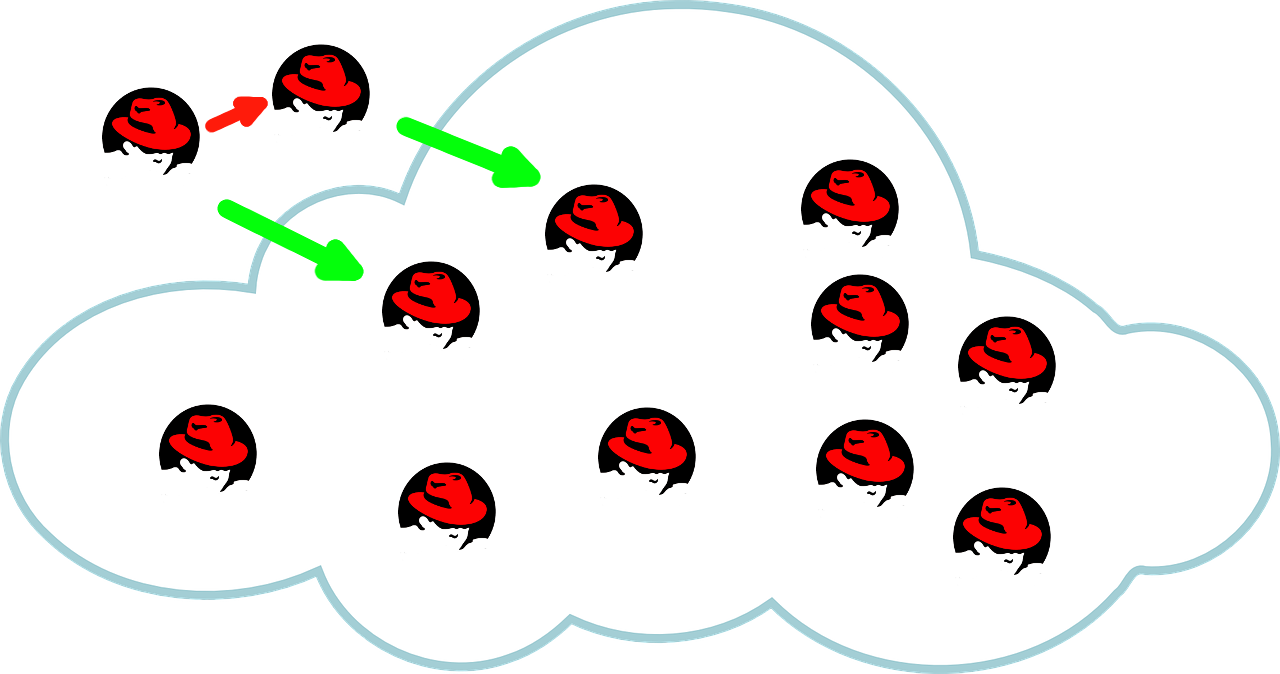
\includegraphics[width=0.8\textwidth]{outofbandwrite.png}
\end{figure}

For example, a pair of clients could be separately accessing a pair of
data objects in the Ceph file system (see
Figure~\ref{fig:out-of-band}). These clients could both be acting on
behalf of the same application. Let's say the application is a text
editor. The application may read from (or write to) a text file
through the first client.  As a result of this operation, the
application then may decide to write to the second text file through
the second client. Since these operations are handled by separate
clients, Ceph cannot be certain of a causal relationship between the
two events.

In addition, Ceph is a very performant system. Currently, writes to a
Ceph cluster take 4 to 20 milliseconds to perform~\citep{Sage}. Any
solution that we provide must maintain Ceph's performance, which means
that its read/write capabilities cannot be interrupted for extended
periods of time.

Finally, Ceph allows a user to use any commodity hardware when
constructing their cluster. This gives users more versatility, but
adds extra constraints on our problem, since we cannot specify
hardware that the user must purchase for a solution to work.

\section{Consistent Snapshots}

A solution to this problem will require recording the global state of
the data in a Ceph cluster. A recording of that global state is called
a ``snapshot". However, we require that a snapshot be consistent.  A
consistent snapshot is one that preserves the causal relationships of
the read/write events that it captures. This means that, if an event
is captured, then all events that caused that event must be captured
as well.

For example, let's say some event $A$ caused some event $B$.  Then a
consistent snapshot is one where, if event $B$ is captured, then event
$A$ is captured as well. If event $B$ were captured, but event $A$ was
not, then any backup based on that snapshot could cause errors in
applications that are using that inconsistent data. See
Figure~\ref{fig:consistency} for examples of consistent and
inconsistent snapshots.

\begin{figure}[!htbp]
  \centering
  \caption{~Event A caused event B. The dashed line in the center represents the time when the snapshot took place. The first three cases are examples of consistent snapshots. The last case is an inconsistent snapshot.} 
  \label{fig:consistency}
  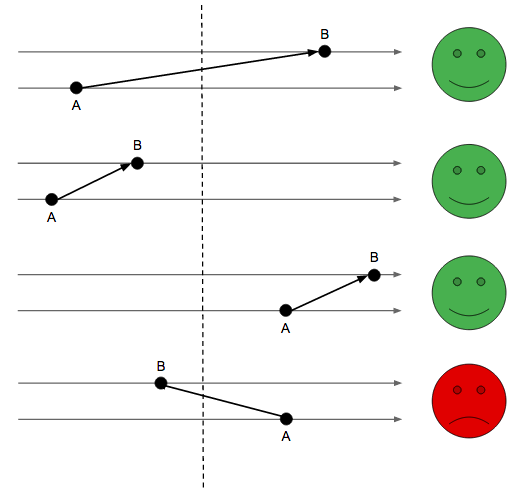
\includegraphics[width=0.75\textwidth]{consistency.png}
\end{figure}

\section{Snapshotting Complications}

The constraints described above make a snapshotting system not as
intuitive as it may initially seem.

Ceph's distributed architecture and lack of central log means that
there is no centralized place where we could obtain a total ordering
of the events in our cluster. A total ordering is an exact order of
all events. Events are logged on the individual nodes. This means that
we will have to use the partial data at each node to reconcile the
ordering of the events, while still maintaining the consistency of the
data in the system.

Logical clocks, like Lamport or vector clocks, are sometimes used to
order events in distributed systems. They provide a partial ordering
of the events in our system, which is where events that have a causal
relationship can be ordered. Ordinarily, these solutions could provide
us a way to order events to construct a consistent snapshot. However,
they fail when out-of-band communication is permitted. Since Ceph
allows for out-of-band communication, Lamport and vector clocks will
not work. For a more detailed explanation of Lamport and vector clocks
and why they do not solve our problem, see Chapter~\ref{sec:rel-work}.

We could also try to achieve ordering through timestamps. In theory,
this would be able to provide a total ordering of events. However,
clocks are not perfect. Over time, clocks drift and become more
desynchronized from each other. Ceph's distributed design means that
each clock uses its own clock when determining the timestamp of an
event. Using the timestamps by themselves will not allow us to get a
total ordering of the events, since the clocks would slowly become
more and more desynchronized, until the clocks are no longer reliable
ways to distinguish when events occured on different nodes. An event
could receive a later timestamp than an event it caused, which could
create an inconsistent snapshot of our system.

Time synchronization protocols like the Network Time Protocol (NTP)
could help keep the clocks in our system from desynchronizing too
greatly. However, no time synchronization protocol we've been able to
find can maintain clock synchronization well enough that would allow
us to use timestamps alone to order events consistently. However, we
will see in Chapter~\ref{sec:approach} that other aspects of time
synchronization protocols will prove useful for our problem.

Another naive approach is to propagate a write freeze throughout the
cluster.  When a specific node determines that it is time to take a
snapshot, it holds all incoming writes and messages its neighbors to
do the same. This message is then sent through the center as each node
does the same. In the end, when all nodes have frozen, the snapshot
can be taken and the nodes begin to unfreeze.

However, depending on the size of the cluster, it could take a long
time for that freeze to propagate through the cluster. If a client
wanted to write to the node that started the freeze, it could take
tens of milliseconds to do so.  This would noticeably degrade Ceph's
performance, which is not acceptable.  However, we will see in
Chapter~\ref{sec:approach} that we can modify this approach to remove
the performance degradation.

Finally, Google has implemented a library called TrueTime to provide
ranges of what real time could be in their Spanner database. While
this solution may seem like it could work, it actually requires
specific hardware, namely atomic and GPS clocks, to function
properly. Since Ceph can be running on any commodity hardware, we do
not want our solution to require specific hardware (though, as we'll
see in Chapter~\ref{sec:impl}, specialized hardware can improve the
performance of our solution). Therefore, we cannot use TrueTime as a
solution to this problem. For a more detailed explanation of TrueTime
and why it does not solve our problem, see Chapter~\ref{sec:rel-work}.

% distributed architecture and no central log
% clock drift and timestamps
% logical clocks and out-of-band
% commodity hardware and true time















%%% Section 3

\chapter{Approach}
\label{sec:approach}

All time synchronization algorithms have some inherent error, because
it is not possible to perfectly match time across a network. Some
algorithms are able to provide an uncertainty that upper-bounds that
error. The most common NTP implementation, ntpd, supports precisely
this. Specifically, it uses packet round trip time between clients and
the NTP server to provide an upper bound on error. It performs very
well with good clocks and network links, but degrades gracefully when
those are absent (see Chapter~\ref{sec:results} for a detailed
investigation of this point). This snapshot algorithm relies on having
a time synchronization algorithm capable of providing upper bounds.


\section{Phases}
There are four phases involved in this algorithm:

\begin{enumerate}

\item \emph{Synchronization}

  During the synchronization phase, all nodes run a supported time
  synchronization algorithm. All nodes attempts to synchronize their
  internal clocks with a single, common master
  clock\footnotemark. Administrative messages are also exchanged
  during this phase. These messages include scheduling future snapshot
  times. These messages could be inserted into already-extant messages
  such as heartbeat messages.

  \footnotetext{Multiple NTP servers may also be used, but they must
    all synchronize to the same root, or \textit{stratum 1}, NTP
    server. Otherwise, the NTP uncertainties will not necessarily
    provide overlapping freeze windows}

\item \emph{Freeze}
  
  When a node is frozen, it holds write confirmations. Incoming writes
  may be processed, but completion is not acknowledged until the end
  of the freeze.
  
  Let $U_i$ be the uncertainty in node $i$'s current time (i.e. the
  error bounds the time synchronization algorithm is able to
  determine), and $T$ be the scheduled snapshot time. Node $i$ begins
  its freeze when its clock reads $T - U_i$, and completes it when its
  clock reads $T + U_i$, guaranteeing that the master clock's $T$ is
  captured in the freeze window for all $i$ (Chapter~\ref{sec:proof}).

\item \emph{Confirmation}

  Before a snapshot may be marked as successful, the data center must
  wait a short period. This allows any sudden clock desynchronization
  events or node failures to be detected and consistency checked. The
  Ceph cluster must verify that, for every node failure during the
  snapshot, at least one other replica of that node's data did not
  fail. This is enough data to recover a snapshot
  (Chapter~\ref{sec:proof}).  If no uncrecoverable inconsistencies are
  found, the snapshot is marked as successful.

\item \emph{Replication}
  
  Finally, the data in the Ceph cluster as it existed at the time of
  the snapshot may begin being replicated to a remote Ceph cluster
  (provided the confirmation phase succeeded).  The first step in
  taking a snapshot is simply writing down a marker in a node's log
  separating pre- and post-snapshot writes. It is therefore
  straightforward either to do a full snapshot, or just capture the
  difference since the last good snapshot (the last snapshot
  log-marker).
  
  While replication is underway, the next synchronization phase begins.

\end{enumerate}

By using the uncertainty in a time synchronization algorithm in this
manner, we are able to have a per-node \textit{safety buffer} in each
freeze period, as shown in figure~\ref{fig:safety-buff}.

\begin{figure}
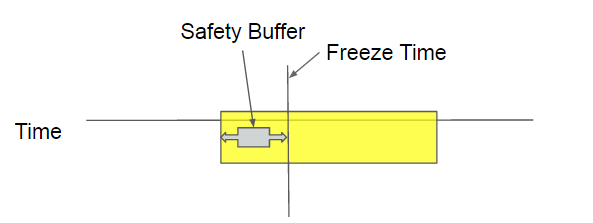
\includegraphics[width=0.8\textwidth]{safety-diagram.png}
\caption{~The gap between the edge of the freeze window and the point at which the NTP server believes the snapshot is scheduled is called the safety buffer}
\label{fig:safety-buff}
\end{figure}

\section{Overlapping freeze windows}

The freeze windows for our algorithm are designed to ensure
that there is some point in time at which all nodes in the cluster are
frozen. Each node knows the intended freeze time. However, since their
clocks are not perfect, they cannot know exactly when they have reached it.

Recall that our algorithm calls for each node to start its freeze
window when its clock reads $T - U_i$, and completes it when its clock
reads $T + U_i$, where $T$ is the freeze time and $U_i$ is the time
synchronization method's (e.g. NTP) uncertainty at that time.  Since
our chosen time synchronization method guarantees that the real time
$T$ will be within the uncertainty bounds of when the node's clock
reads $T$, we can be sure that each node will be frozen when the NTP
server's clock shows the scheduled snapshot time. Therefore, we can be
certain that their freeze windows overlap.
Figure~\ref{fig:overlapping-windows} demonstrates this concept with
four freeze windows overlapping at the freeze time of 8pm.

\begin{figure}[h]
  \centering
  \caption{}
  \label{fig:overlapping-windows}
  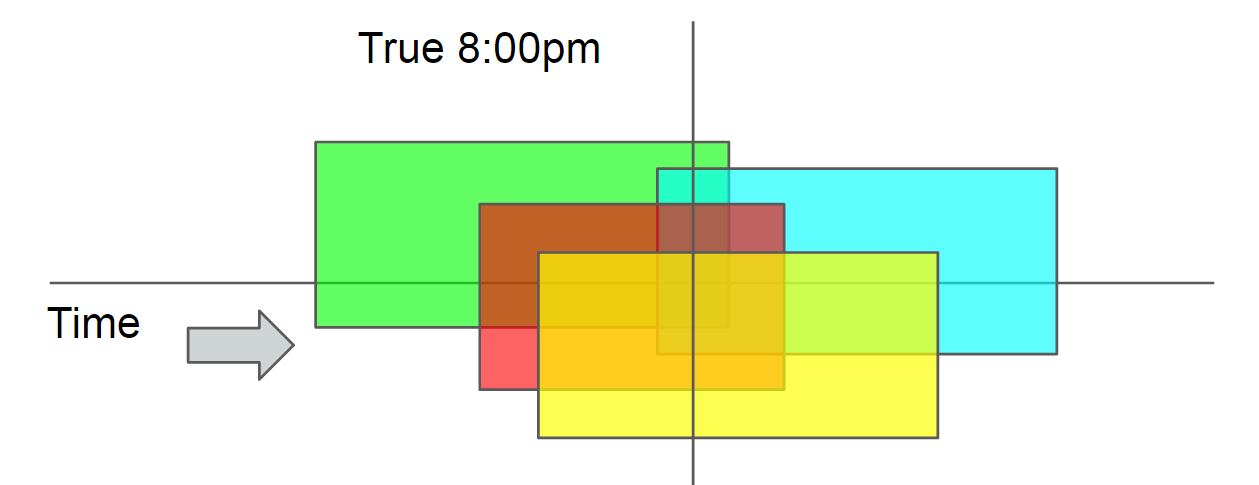
\includegraphics[width=0.8\textwidth]{overlapping-windows.png}
\end{figure}


%%% Section 4

\chapter{Related Work}
\label{sec:rel-work}

Creating a consistent snapshot of a Ceph cluster is difficult because
Ceph is distributed: The system does not have a single or small group
of nodes that can track every transaction. Instead, the cluster must
aggregate knowledge from potentially thousands of nodes to capture a
complete point-in-time snapshot of its data.  Significant research
efforts have been directed toward taking snapshots as well as
synchronizing and ordering events in distributed
systems. Unfortunately, none of these approaches can address the
particular constraints of Ceph outlined in Chapter
\ref{sec:description} without modification.

\section{Logical Clocks}

Lamport clocks use a ``logical clock'' to establish a partial ordering
of events in distributed systems. If an ordering of the events and
messages between nodes in a distributed system can be established, and
this ordering is complete enough to take into account all
dependencies, a snapshot may be obtained by observing which events
happen before other events.

Lamport clocks try to order events and messages by a logical
timestamp, a counter that increments following each event or message
pass, rather than by some physical time that could be affected by
clock drift. This ordering method works well if the system can reason
about events that are occurring between its own nodes. However, this
type of partial ordering fails to guarantee correct ordering in the
case of out-of-band communication as described in Chapter
\ref{sec:description}; the system cannot order the events that occur
outside of the system as it has no knowledge of the order of those
events. These clocks might still be useful for reasoning about
interactions that occur strictly within the Ceph cluster, but they
require a second system that supports out-of-band communication to
meet Ceph's consistency guarantee~\citep{Lamport1978}.

Vector clocks are very similar to Lamport clocks. Instead of
maintaining a single logical time, each node stores a vector of
times. Each element of the vector represents other nodes in the
system.  The value of each element is the time of the last event
received by that given node in the system. The ordering of events is
based on the relative times stored in the vectors. All messages
contain the sending node's vector and a node updates its vectors when
it receives a message. Vector clocks can be superior to Lamport clocks
for some purposes because they do not assign an arbitrary counter
representing time to events. Instead, they use the relative times of
to other nodes to determine the partial order of the events. However,
like Lamport clocks, out-of-band communication is not accounted for
and events could be incorrectly ordered~\citep{Fidge1988}.

\section{Network Time Synchronization}

As mentioned in Chapter \ref{sec:description}, total ordering can be
achieved through timestamps. In theory, this would be able to provide
a total ordering of events including any out-of-band
communication. Clock drift and skew complicate this approach: When
multiple clocks are in use in a distributed system, the clocks must be
synchronized in order to use timestamps to order events across nodes.

A synchronization algorithm could be effective should it provide
sufficiently tight, provable bounds on the drift of a given clock and
on the skew across the distributed system. These bounds provide a
method to obtain a consistent snapshot as we described in our
algorithm in Chapter \ref{sec:approach}.

Many clock synchronization algorithms already exist. However, these
algorithms tend to have major shortcomings when they are considered
for application to this problem within a data center. A
synchronization method must have bounds on the clock error in order
events in a snapshot, and these error bounds must also be a hard upper
bound in order for Ceph to make guarantees about the consistency of
its snapshots. The following subsections describe different time
synchronization methods and protocols.

\subsection{Network Time Protocol}

NTP is a robust algorithm for time
synchronization~\citep{Burbank2010}. NTP is designed to synchronize
time at geographically separated computers over the internet. As a
result, it is resilient to node failure, network unreliability, and
poor clock quality. NTP requires very little information about the
network configuration and nodes on which it is operating to provide
useful synchronization. NTP uses statistical estimators to predict
future clock performance. Notably, NTP does define a maximum error
term in relation to a single root time source. Given this maximum
error term, NTP is a potential choice as a time synchronization method
in our algorithm.

A better solution is possible, however. NTP's focus on robustness
causes compromises for the freeze time. NTP consistently overestimates
uncertainty (see Chapter~\ref{sec:results} for an in-depth examination
of this issue). A protocol designed for local area network
synchronization could likely do away with some of the complexity of
NTP, make more assumptions about network configuration, and as a
result provide tighter bounds on its error.

In Chapter~\ref{sec:results}, we analyze the performance of an NTP
implementation, \texttt{ntpd}, across various clock and network
conditions. The \texttt{ntpd} daemon was chosen for its common use and
ease of access to relevant calculated parameters. \texttt{Chrony} is
another potential choice for an NTP implementation, although it lacks
some diagnostic
reporting. %% TODO these were flagged as needing citations
                      %% but I'm not convinced we really need them?

\subsection{Precision Time Protocol}

Precision Time Protocol (PTP) is designed for tightly synchronizing
computers on a local network ~\citeyearpar{2008}. To gain even better
synchronization with tighter bounds on clock uncertainty than NTP, a
user may use specific hardware that supports PTP. Hardware that
supports PTP is generally included in current data center switches
already. The type of hardware that supports PTP helps decrease the
amount of random variation in message latency in a network, enabling
extremely accurate measurements of time.  These measurements should in
theory provide extremely tight uncertainty bounds. However, the
protocol does not specify (and the implementation does not include) an
upper bound error value. This means that this protocol is not
currently suited for use with our algorithm.

If performance of NTP is found to give unsatisfactory clock
uncertainty bounds, it would be worth considering extending PTP to
give an upper bound uncertainty value (Chapter~\ref{sec:impl} has a
brief discussion of this). The implementation of a maximum error term
would be sufficient for PTP to be used with our algorithm.

% NOTE: Don't think these are needed. Awkward to add implementation details 
%     into related work
%Linux PTP is an implementation of the Precision Time Protocol 
%(PTP)~\citeyearpar{2008}. PTPd is another
%implementation~\citeyearpar{2008}.

\subsection{Wireless Synchronization}

Surprisingly, wireless time synchronization is a much easier
problem. Wireless signal propagation times are easy to model and as a
result time synchronization is easy to perform with a high level of
accuracy. Protocols such as PulseSync take advantage of this
observation to achieve highly synchronized clocks~\citep{Lenzen2010}.

If highly synchronized clocks are a requirement, a wireless
synchronization protocol could be designed that would allow for a high
level of confidence on the clock uncertainty bounds.  This would
require specialized hardware, and one of the goals of this project is
to provide a solution that can work on any commodity hardware.

GPS Synchronization is a special case of wireless synchronization that
can provide a nearly perfect time source around the world. It is
advisable to incorporate a GPS time source (or similarly accurate time
source) into the master clock of any implementation of our algorithm
in order to achieve tighter uncertainty bounds, though adding this
would require specialized hardware.  The details of this are discussed
in Chapter~\ref{sec:impl}.

\section{TrueTime}

Google has a number of time-sensitive applications, such as the
synchronously geo-replicated Spanner database. Synchronous
geo-replication of database transactions requires very strong time
guarantees because database transaction ordering is important for
reliability and security.

A library called TrueTime was developed to support these applications.
TrueTime does not provide current time in the way that standard time
libraries do, such as for NTP or PTP. Instead, the ``current time'' it
gives is a range that is guaranteed to contain the real current
time. The bounds are claimed to be generally less than 10
milliseconds. This range in the real current time allows for rapid
throughput on the database while still maintaining definitive
transaction ordering. When TrueTime's guaranteed bounds start to
spread, it will throttle writes to maintain that
ordering~\citep{Corbett2012}.

TrueTime relies on having extremely accurate and precise clocks to
maintain sub-10ms skew between geographically diverse data
centers. Specifically, Google has placed atomic and GPS clocks in
their data centers. TrueTime runs a daemon that talks to these clocks,
both in its own data center and in others. TrueTime is able to weed
out clocks whose timing information is not reliable (e.g. due to
network latency)~\citep{Corbett2012}.

TrueTime is a proprietary library that requires special hardware, thus
it would not be able to be used directly as a solution to Ceph's
asynchronous replication problem.

%% NOTE: If we are going to talk about this, we need more information
%% However, if a similar open source protocol became available,
%% it could merit deeper analysis. %% TODO This exists, we talked about
                                %% it, it's called Cockroach


%%% Section 5

\chapter{Proof of Theoretical Consistency and Performance}
\label{sec:proof}

Since Ceph makes strong consistency guarantees, CASTS must provide a
theory-justified guarantee that, in the absence of a hardware failure,
snapshots taken according to the procedure described in
Chapter~\ref{sec:approach} will always be consistent. Further, because
Ceph is a data center file system, CASTS must be performant. The first
step toward demonstrating performance is a theoretical description of
its performance characteristics.

\section{Consistency}

As described in Chapter~\ref{sec:description}, a snapshot would be
inconsistent if it captured an event, $X$, but not an earlier event that
caused $X$. To provide an intuitive example, let $A$ be some event that
caused another event, $B$.  For example, $A$ could be a new user added
to a database. Event $B$ could be a change to another user's friend
list to include $A$. If we captured $B$ in our snapshot, but not $A$,
our snapshot would contain the friend relation, but not the new
user. Recall the examples provided in Figure~\ref{fig:consistency} for
a visual demonstration of what this would mean.

More formally, here is the statement that we want to prove: {\em let
  $A$ and $B$ be events in our system, where $B$ was caused by
  $A$. Our goal is to prove that if $B$ was captured in our snapshot,
  then $A$ must have been as well.}

This is equivalent to the visualization provided by
Figure~\ref{fig:consistentoverlap}.

\begin{figure}[!htbp]
  \centering
  \caption{All possible event orders given that A caused B. Yellow and green boxes are node freeze windows for two different nodes, and the dotted blue line is the overlap when the snapshot is taken. We can see that B is captured only if A is captured.}
  \label{fig:consistentoverlap}
  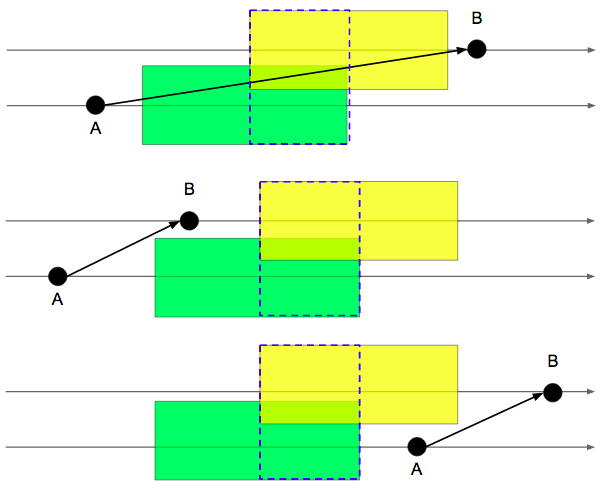
\includegraphics[width=0.75\textwidth]{consistentoverlap.png}
\end{figure}

First, define $T_A$ to be the (objective) time at which $A$ occurred
and $T_B$ to be the (objective) time at which $B$ occurred. Since $A$
caused $B$, we know that $A$ must have taken place before $B$, meaning
$T_A < T_B$.

In Chapter~\ref{sec:approach}, we shows that CASTS guarantees that all
of the freeze windows of the nodes in our system will overlap when we
are taking a snapshot. In other words at some point in time or for
some time period, all nodes will be frozen.  During this interval, the
cluster as a whole will not confirm completion of to write events. For
clarity, when we are considering the order of events, we will collapse
the entire freeze window into a single event $F$ and consider the start
time of the interval to be the time of the event $T_F$.

Suppose by way of contradiction that there is a series of
events that could violate the invariant that an event would only be
captured in a snapshot if all events that caused that event were
captured as well. More specifically, let us have events $C$ and $D$
such that $C$ caused $D$. Assume that it is possible for $D$ to have
been captured in the snapshot while $C$ was not.

Recall from Chapter~\ref{sec:approach} that each node's portion of the
snapshot occurs when that node first freezes. No other events will
occur on that node between when it takes its snapshot (i.e., the
beginning of its freeze interval) and $F$, the moment when all nodes
are frozen. By our assumption above, if $D$ was included in the
snapshot, it must have happened before $F$, meaning $T_D <T_F$. Since
$C$ caused $D$, it must have happened temporally before $D$.  Since
$C$ was not captured in the snapshot, it must have happened either
after $F$, or between its node's freeze start time and $F$. The first
is clearly a contradiction, since $D$ happened before $F$. The second
is a contradiction, because then $C$ would not have completed before
$F$, so it could not have caused anything before $F$. So, we know that
our original assumption that $D$ was captured and $C$ was not must
have been incorrect. Therefore, our statement must be true for any
pair of events in the cluster that are causally related. Since our
statement is true for any two events in our system with a causal
relationship, we know that our snapshot must be consistent.

\section{Theoretical Performance}

There are several performance characteristics that need to be
considered to preserve Ceph's performance when implementing a
snapshotting algorithm. First, we need to consider the impact of
delaying writes for a freeze. Since each node freezes for twice the
uncertainty bounds that is determined by the time synchronization
protocol, the magnitude of the uncertainty bounds is dependent on
which protocol is used. In Chapter~\ref{sec:results}, we analyze the
uncertainty that NTP provides and discuss what impact CASTS would have
on a Ceph cluster if NTP is used as the time synchronization
protocol. However, as long as a time synchronization protocol could
provide uncertainties in the 5-10 millisecond range, yielding 10-20
millisecond freeze windows, our algorithm should not impact the
cluster's performance in a way noticeable to client
applications~\parencite{Sage}. Also, each node's freeze window is
offset from other nodes', because each freezes for its own individual
uncertainty bounds, so the period of time for which the whole Ceph cluster is
frozen is much.

In this section, we consider the impact of network link quality on
this algorithm. We need to be assured that our algorithm does not
require significant amounts of bandwidth which would cause network
congestion within a Ceph cluster. Since most Ceph clusters are already
running a time synchronization protocol like NTP, our algorithm does
not require any extra messages during the synchronization phase. The
freeze phase also does not require any extra messages. The number of
success/failure messages required in the confirmation phase is $O(n)$
in the size of the cluster and thus would not have an excessive impact
on the performance of the cluster (because each message would be only
a few bytes). In the replication phase, the remote cluster needs to
read the data from the local one, but this cost is inherent to any
snapshotting algorithm.

Finally, we need to consider whether CASTS, will place a significant
computational burden on nodes. Each primary node needs to send its
data to the remote cluster. This should not impact the performance of
the primaries, since it should only take a small amount of time for
each to send its data provided data is sent in differences between
snapshots rather than complete sets. Even if it did take some time to
send the data, read and write requests could still be addressed by
prioritizing those requests above the requests for the objects from
the remote cluster. Sending all of the data out at once could require
nontrivial bandwidth. Since it is distributed throughout the Ceph
cluster, however, the bottleneck would be the bandwidth from the local
cluster to the remote cluster. The inter-cluster pipe should be
large and not a concern if we prioritize normal client traffic over
the inter-cluster traffic.

Based on our analysis, our algorithm should not degrade the
performance of a Ceph cluster.


%%% Section 6

\chapter{Testing and Analysis}
\label{sec:results}


With a theoretical proof of CASTS, we can move on to testing
and analyzing its real-world tractability and performance in creating
small freeze windows.  Key to
this endeavor, we must establish that any time synchronization
protocol we choose is capable of reporting correct and accurate
uncertainties for a node's time. As these uncertainties are used in
calculating freeze windows, they must contain the real time
(correctness), yet be small enough for CASTS to be performant
(accuracy).

For the purposes of this project, we chose to make an in-depth
analysis of the NTP implementation \texttt{ntpd}. NTP is an
off-the-shelf protocol. Choosing an off-the-shelf protocol would
greatly simplify implementation of CASTS in Ceph. Of the
protocols we investigated in Chapter~\ref{sec:rel-work}, NTP is the
only general purpose, open source protocol that has the
functionality of providing the uncertainty bounds on clock error 
that CAST requires. Its robust
design also suggests that it can function well in environments
consisting of commodity components, as many Ceph deployments do. 
Given these observations, NTP and \texttt{ntpd} were
clear choices for a close analysis.

We want to determine whether \texttt{ntpd} can correctly and
accurately report each node's uncertainty. By monitoring \texttt{ntpd}
on a Ceph cluster, we can gain a sense of the accuracy of uncertainty
reporting, along with many other statistics. However, in the real
world we have no way of measuring the true difference in time
between a given node and its NTP server. If we had a way of obtaining
this measurement, the task of synchronizing clocks would be trivial
as we could achieve perfect synchronization without any uncertainty.
Thus, the task of testing correctness by comparing nodes' clocks to a
reference clock in the real
world is impossible. As a result, simulations will factor heavily into
our analysis of \texttt{ntpd}.

This chapter is split into two sections. The first section discusses
data collection on a Ceph test cluster. This section also details how
the collected data can be used to improve the testing of \texttt{ntpd}
in simulations.  The second section describes the setup of the
simulations of nodes and their clocks and analyzes the results of those
simulations. It seeks to verify that the measurements and values
\texttt{ntpd} reports are reasonable, correct, and accurate. This
section includes a discussion of the performance of the uncertainty
provided by NTP under various network
conditions.

We show that NTP and \texttt{ntpd} are a capable algorithm and
implementation for the purpose of time synchronization.  
The \texttt{ntpd} program will provide correct values
under any reasonable network configuration. However, a low-latency
network will ensure best performance. In ultra low-latency
environments, an alternative protocol should be explored to take advantage
of the possibility of having smaller uncertainty bounds and as a result, 
smaller freeze windows. NTP's conservative
assumptions of maximum possible error, result in a
minimum uncertainty on the order of a millisecond.



\section{Measuring \texttt{ntpd}'s Performance in the Real-World}

In order to accurately simulate the characteristics of a real Ceph
cluster to test \texttt{ntpd}, we need to model the behavior of a
Ceph cluster.

To observe how \texttt{ntpd} interacts with a live Ceph cluster, we
logged diagnostic data, described below, on a test Ceph cluster 
for a period of months.
The test cluster on which we logged data includes three
classifications of computers, named here Mira, Plana, and
Burnupi. Mira and Plana use Intel-based chips, while Burnupi uses
AMD chips.

Of the diagnostic data being logged, we considered two parameters of
interest: clock frequency offset and network latency.  The
frequency offset is the estimated random error on a given node's clock
drift in comparison to the NTP server, and is typically measured in
Parts Per Million (PPM). For example, a clock frequency offset
measurement of 10 PPM means for every million clock ticks of the
NTP server, the local
%TODO: is this really freq offset? Is there a better way to describe it?
node's clock could be off by 10 ticks. The network latency is a
measure of the round trip time of the message passed between a local
machine in the Ceph cluster to the NTP server and back. The round trip
time is typically on the order of single-digit milliseconds~\citep{Sage}.

%TODO: Do we need 4 sig figs here? I doubt we can claim more than one or two...
The histogram in Figure~\ref{fig:latency-hist} shows the logged values
of network latency in the cluster. The difference in network latency
between each type of machine is not statistically significant, as we
would expect given that the network latency between machines should
not depend on the type of machines in the network.
%TODO: Did you actually do a p-test? Do you have a significance level if you did?

\begin{figure}[h]
  \centering
  \caption{~Histogram of network latency across 234 nodes in a Ceph test cluster. The mean is 2.7 ms, the 
  standard deviation is 10.3 ms, and the median is 0.6 ms.} 
  \label{fig:latency-hist}
  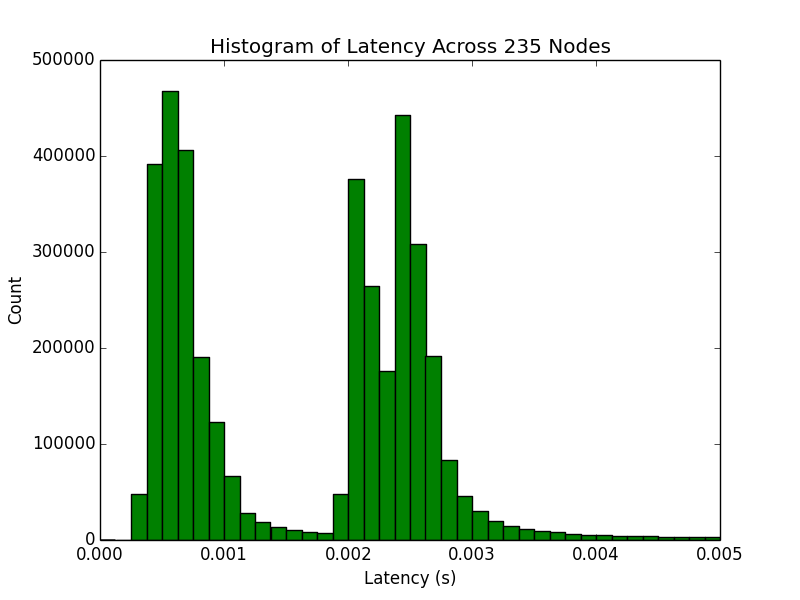
\includegraphics[width=0.8\textwidth]{latency-hist.png}
\end{figure}

\begin{figure}[!htbp]
  \centering
  \caption{~Histogram of NTP's frequency offset for Burnupi machines in the Ceph test cluster.
  The average frequency
  offset for individual Burnupi machines is -5.2 PPM with average
  standard deviation 1.1 PPM.}
  \label{fig:burnupi-hist}
  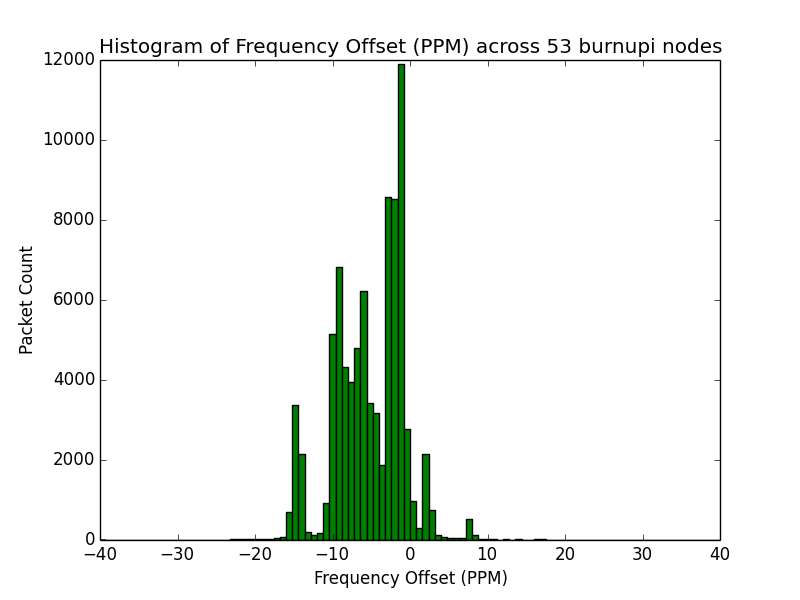
\includegraphics[width=0.8\textwidth]{burnupi-freq-offset.png}
\end{figure}

\begin{figure}[!htbp]
  \centering
  \caption{~Histogram of NTP's frequency offset for Mira machines in the Ceph test cluster.
  The average frequency offset for individual Mira machines is 10.8 PPM with average
  standard deviation 0.4 PPM.}
  \label{fig:mira-hist}
  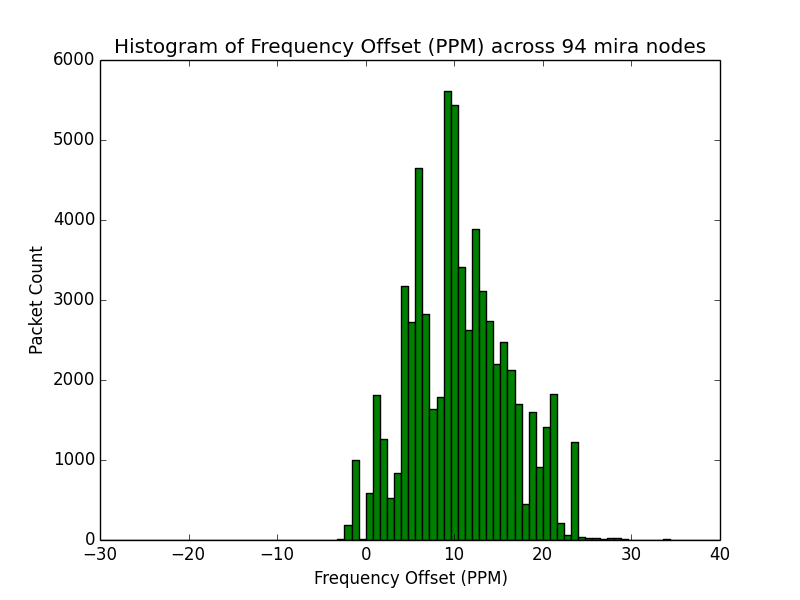
\includegraphics[width=0.8\textwidth]{mira-freq-offset.png}
\end{figure}

\begin{figure}[!htbp]
  \centering
  \caption{~Histogram of NTP's frequency offset for Plana machines in the Ceph test cluster.
  The average frequency offset for individual Plana machines is 13.3 PPM with average
  standard deviation 1.7 PPM.}
  \label{fig:plana-hist}
  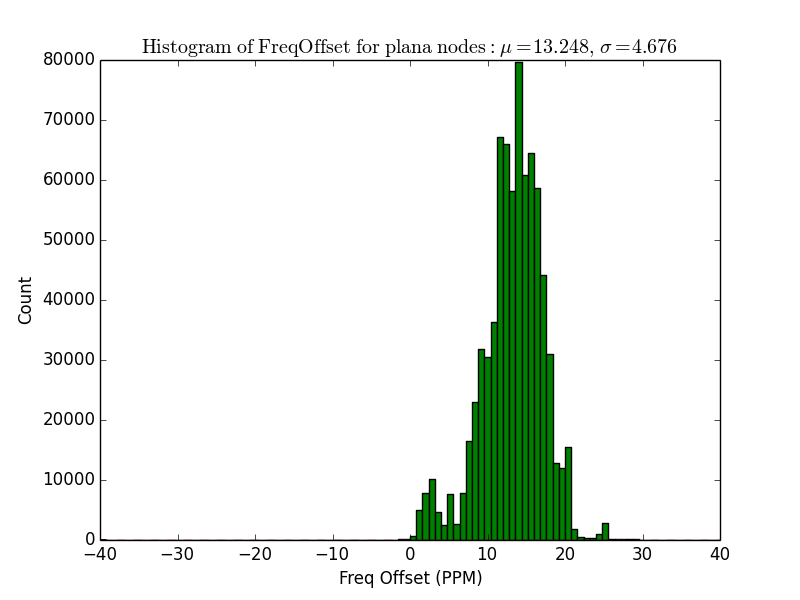
\includegraphics[width=0.8\textwidth]{plana-freq-offset.png}
\end{figure}


Figures~\ref{fig:burnupi-hist},~\ref{fig:mira-hist},
and~\ref{fig:plana-hist} show the behavior of clock frequency offset
on the three types of machines in the Ceph cluster. The distribution of frequency
offsets on all three types of machines are consistent with a 
normal distribution. The average standard deviation across all
nodes is 1.033 PPM, and the mean values of each type are reasonable as we would 
generally expect frequency offset to be at most $\pm 20$ PPM~\citep{gregscott}. 
It is interesting to note that the Burnupi
machines with the AMD chips have primarily negative clock frequency
offset, while the Mira and Plana machines with Intel chips have
primarily positive clock frequency offsets.



        



\section{Analysis of Simulation of NTP}

With the data collected on frequency offset and network latency, we
can now simulate a test cluster with input parameters that reflect the
real world. Recall that we cannot simply use a real Ceph
cluster to observe overlapping freeze windows because there is no
way to observe the real time on a given computer. A simulated network
environment running on a single computer has the advantage of having a
single clock on which all simulated clocks are based. By having a
single clock, we are able to quantify and verify the claims that time
synchronization protocols make about the quality of a synchronization
and the quality of the clocks involved.

%TODO:
% NOTE: I'm not sure this paragraph is needed?
% By using a simulation that abstracts the clock from a physical clock,
% we also eliminate any potential for idiosyncrasies of the host system
% clock to affect the measurements gathered in the simulation. This has
% the added benefit of allowing the simulation to run at a speed much
% greater than real time.
We have chosen to use an environment called
\texttt{clknetsim} %TODO reference to clknetsim repo?
to conduct our simulations. The open-source simulation package
\texttt{clknetsim} is developed and used by a major contributor to the
\texttt{chrony} project~\citep{chrony} and the \texttt{linuxptp}
project~\citep{linuxptp} to test these protocol implementations. In
comparison to commercial network simulation products, it provides a
simple codebase and feature set targeted at measuring time across a
simulated network. We have made slight additions to and modifications
of the \texttt{clknetsim} package. These extensions were made in order
to expose state parameters of NTP that were not being exposed,
including the maximum error term.

The package \texttt{clknetsim} makes use of the environment variable
\texttt{LD\_PRELOAD} in the Linux library to intercept system calls
that time synchronization libraries make on their hosts. Using these
intercepted calls, \texttt{clknetsim} is able to monitor and capture
the internal state of the synchronization program. It is also able to
fully control the information the host's time library receives from
the network and the system clock. As \texttt{clknetsim} is
manipulating system clocks and network connections for the simulation,
it can shape the behavior of the clock and network parameters to test
different setups and hardware properties.

We are most interested in measuring two parameters in this system. We
first want to determine if the uncertainty bounds reported by NTP is
correct. We can check that the uncertainty bounds report is correct
by ensuring that the uncertainty bounds on a given machine clock's
time includes the real time.  The \texttt{clknetsim} package, for a
given point-in-time in the simulation, allows us to observe what NTP
estimates the time is along with information about how certain NTP is
about that time. Our second goal is to analyze the accuracy of the
time synchronization: the magnitude of the uncertainty.  As 
CASTS is predicated on a upper bound of the uncertainty in time,
performance analysis can be accomplished by observing how modifying
parameters such as network latency affect the uncertainty bounds
that NTP reports.
%TODO: effect?

\subsection{Simulation Using Real-World Parameters}

For each node, NTP has an estimate for the real time and an uncertainty
in that estimate. \texttt{Clknetsim} allows us to access that information, and
it lets us to know the real time of the system. All of this admits
us to know what the ``safety buffer" is for each node in real time.

Recall the safety buffer first introduced in Section~\ref{sec:overlapping}, $S(t)$,  for a particular node is defined as:

\[ S(t) = U(t) - | t - E(t)| \]

where $t$ is the real time, $U(t)$ is NTP's uncertainty in the real
time estimate for that node, and E(t) is NTP's estimate for what the
real time is. In simpler terms, the safety buffer tells us where in NTP's
uncertainty range lies the error from real time (see
Figure~\ref{fig:safety-diag}). If the safety buffer is a positive
value, then the difference between NTP's estimate and real time is
within its uncertainty range. If it is negative, then its error is
outside of its uncertainty range, meaning that NTP does not function as
we would expect.

\begin{figure}[!htbp]
  \caption{~The safety buffer tells us where NTP's error in what the real time is lies within its uncertainty range.} 
  \label{fig:safety-diag}
  \centering
  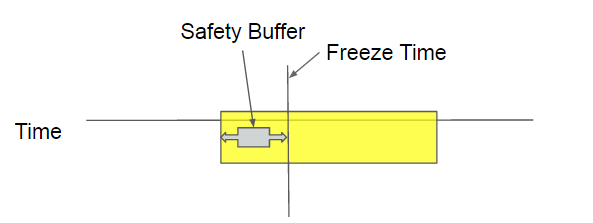
\includegraphics[width=0.5\textwidth]{safety-diagram.png}
\end{figure}

The NTP specification declares that the maximum error it reports is
the uncertainty in the time accounting for error from all
sources~\citep{Burbank2010}.  While running simulations, we monitored
the safety buffer to test if \texttt{ntpd} is implementing the
uncertainty calculation as we would expect and to quantify how much
\texttt{ntpd} overestimates the uncertainty.  When parameterizing the
simulation with latency values recorded from the Ceph cluster, we
observed safety values summarized in Figure~\ref{fig:safety-data}.

We can see that all of these values are positive. The daemon
\texttt{ntpd} does seem to function as expected under the simulation
conditions we observed.

\begin{figure}[!htbp]
  \caption{~Generated from uncertainty data recorded during simulation parameterized
  with latencies recorded during monitoring of Ceph cluster. Uncertainty and time
  data was recorded once per second in the simulation and the included statistics 
  generated from the total dataset after the simulation was allowed to stabilize. 
  The positive values indicate that the real time is occurring within \texttt{ntpd}'s 
  uncertainty interval.}
  \label{fig:safety-data}
  \centering
  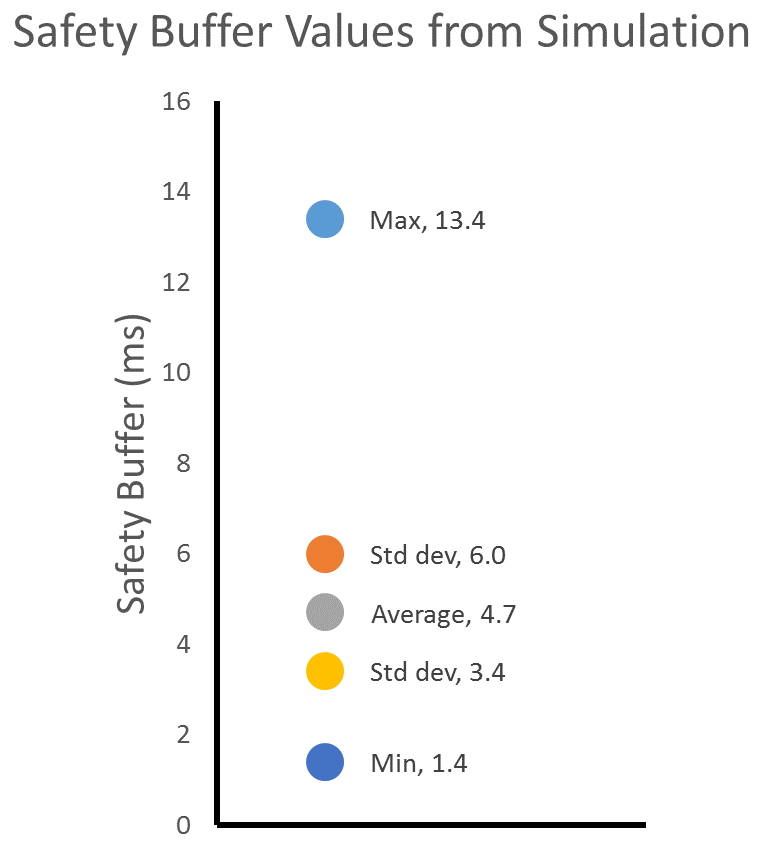
\includegraphics[width=0.55\textwidth]{5pointsSafety.png}
\end{figure}

\subsection{Generalization of Simulation Parameters}

The previous section demonstrated that \texttt{ntpd} functions as we expect in 
a real world scenario.  This section
analyzes \texttt{ntpd}'s performance under a wide variety of simulated
conditions---a wider range of conditions than \texttt{ntpd} would
likely encounter in the real world.  We found that network latency was the 
largest contributer to the uncertainty, though the relationship does not 
continue for ultra-low latency networks.

For these simulations, network latency was modeled using a gamma
distribution,
%TODO: find a citation for this?
since the data from the test Ceph cluster suggests that
latency approximately followed such a model. We varied two parameters:
the mean value and the shaping parameter, or alpha. The shaping parameter 
determines the length of the tail for the distribution: a larger value 
shortens the tail of the gamma
distribution.  A very small shaping parameter value approximates an
exponential distribution and a very large shaping parameter value
approximates a normal distribution.

%% TODO please \ref these somewhere

%% TODO: once we finalize the graphs, we should add some commentary about 
%%       the values we're seeing actually mean.
\begin{figure}[!htbp]
  \caption{~NTP's max uncertainty is plotted vs. the network latency mean and the network latency alpha parameter. We can see that the latency mean has a significant impact on the uncertainty, whereas the alpha parameter only impacts the uncertainty for large latency mean values.}
  \label{fig:max-uncertainty_latency-mean_latency-alpha}
  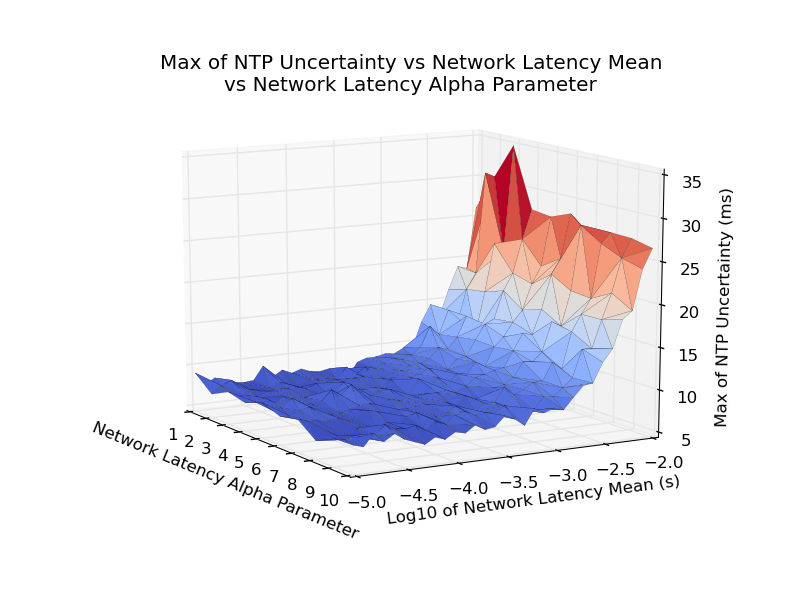
\includegraphics[width=0.8\linewidth]{max_error-latency_mean-latency_alpha.png}

  \caption{~NTP's mean uncertainty is plotted vs. the network latency mean and the network latency alpha parameter.}
  \label{fig:mean-uncertainty_latency-mean_latency-alpha}
  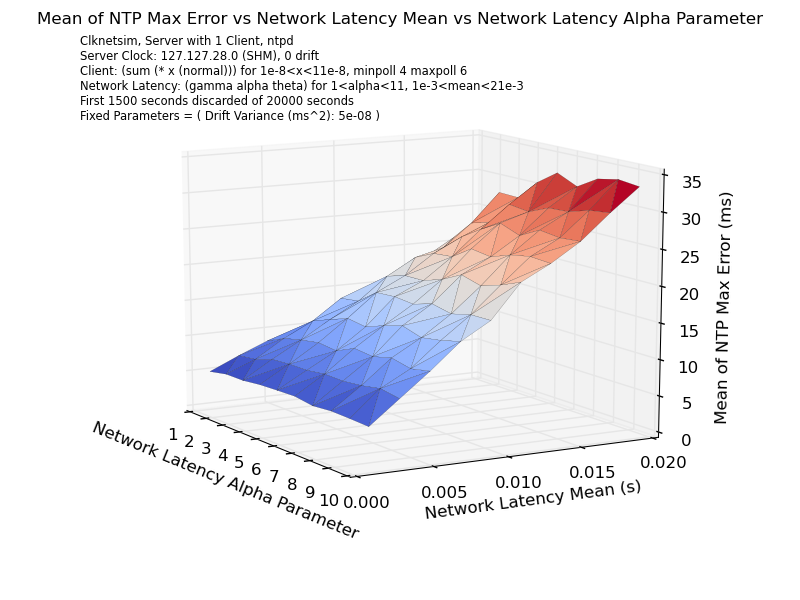
\includegraphics[width=0.8\linewidth]{mean_max_error-mean_latency-latency_alpha.png}  
\end{figure}
%% Put in the appendix
% \begin{figure}[h]
%   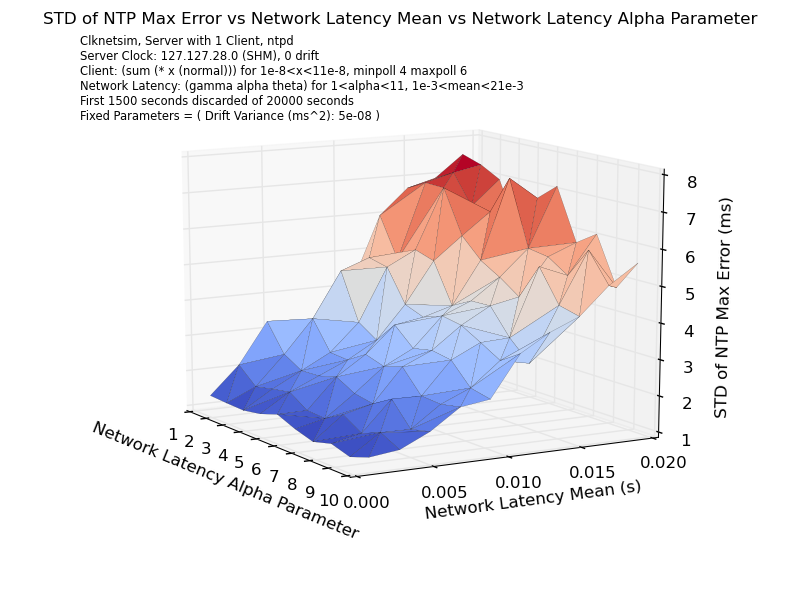
\includegraphics[width=0.8\linewidth]{max_err_stddev-latency_mean-latency_alpha.png}
% \end{figure}

%% TODO: once we finalize the graphs, we should add some commentary about 
%%       the values we're seeing actually mean.

We used the results from the simulations to generate graphs that display the
maximum uncertainty value and the mean of the uncertainty values. In these
graphs, we vary two of the parameters and hold the third constant. 

The maximum uncertainty value observed during a simulation is strongly
affected by the mean network latency. The shape of the latency
distribution has a much weaker effect on the maximum uncertainty
value. A low mean result in a low maximum uncertainty regardless of
the shaping parameter value. A larger shaping parameter value does
have a small effect on the maximum uncertainty. We can see this effect
in Figure~\ref{fig:max-uncertainty_latency-mean_latency-alpha} at the
top right corner.

Interestingly, we see, in Figure~\ref{fig:mean-uncertainty_latency-mean_latency-alpha}, that the mean of the measured uncertainty values
increases with increasing alpha. As alpha increases the distribution of 
latency values is more normal, resulting in more spread out latency values.
When the network
latency distribution has a long tail, most of our latency values will be less
than or below the mean value. Values larger and farther away from the
mean happen less frequently. NTP uses
filtering and prediction algorithms to improve its estimates of the
time~\citep{Burbank2010}. NTP's filtering algorithms likely catch
these anomalous values and ignores them, keeping its uncertainty at a
lower, more reasonable value. We then see lower uncertainty values for
lower alpha values.

\begin{figure}[!htbp]
  \caption{~NTP's mean uncertainty is plotted vs. the network latency mean and the clock's drift variance. We can see that, compared to the latency mean, the clock drift variance has very little impact on the uncertainty.}
  \label{fig:max-uncertainty_latency-mean_drift-variance}
  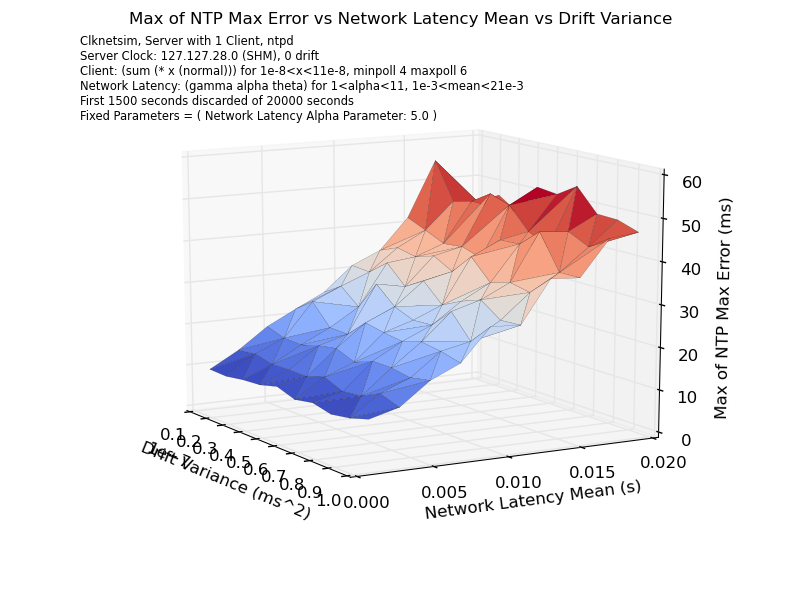
\includegraphics[width=0.8\linewidth]{max_max_err-mean_latency-drift_variance.png}

  \caption{~NTP's max uncertainty is plotted vs. the network latency mean and the clock's drift variance.}
  \label{fig:mean-uncertainty_latency-mean_drift-variance}
  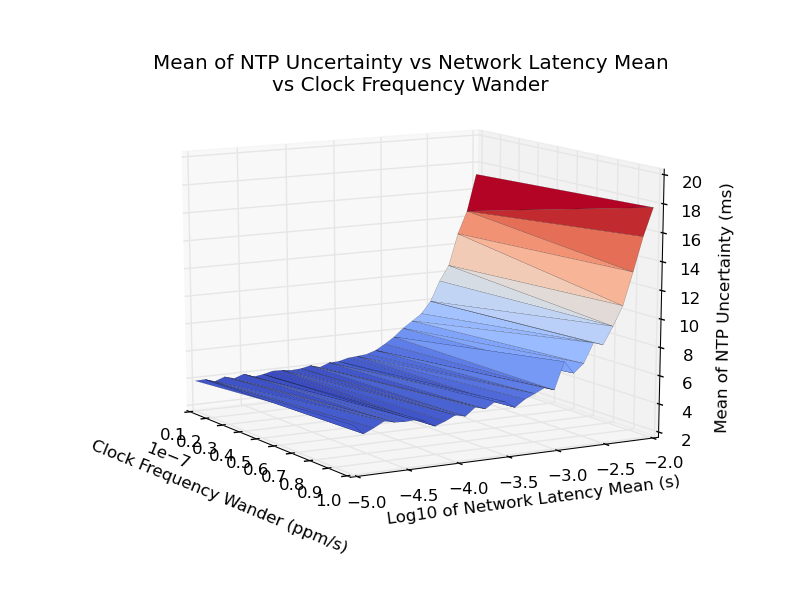
\includegraphics[width=0.8\linewidth]{mean_max_err-mean_latency-drift_variance.png}
\end{figure}

Figure~\ref{fig:max-uncertainty_latency-mean_drift-variance} and
Figure~\ref{fig:mean-uncertainty_latency-mean_drift-variance} show how
clock frequency variation, or clock wander, affects the size of the
uncertainty value.  We can see that there is very little, if any,
effect from a clock's wander on the maximum uncertainty term. The
slope along the x-axis (clock frequency wander) is effectively 0, a
horizontal line. This is expected: network latency is a term with a
much larger magnitude than the wander of even the worst clocks. We do
see a linear correlation between mean latency and the uncertainty term.

In each of these graphs, there is a clear floor: the mean of the
measured uncertainty values does not drop below four
milliseconds, even when the latency mean is tens of microseconds. 
This suggests that NTP will work well in scenarios
involving commodity network hardware where latencies are not necessarily ultra-
low. However, in ultra-low latency scenarios, it may be advantageous to look 
for a protocol that is designed more specifically for a high performance 
network.



%% Put in the appendix
% \begin{figure}[t]
%   \caption{}
%   \label{fig:stddev-mean-drift-var}
%   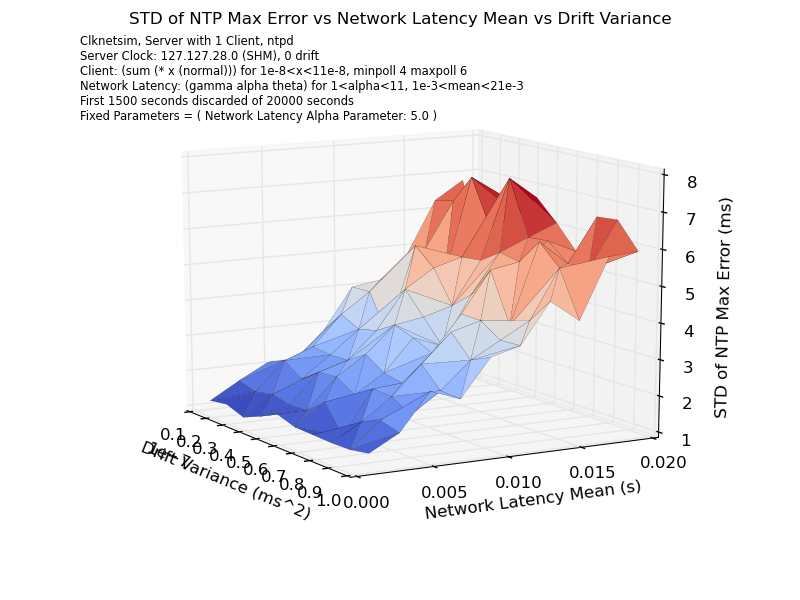
\includegraphics[width=0.8\linewidth]{stddev_max_err-mean_latency-drift_variance}
% \end{figure}

%% Put these figures in an appendix
% \begin{figure}[h]
%   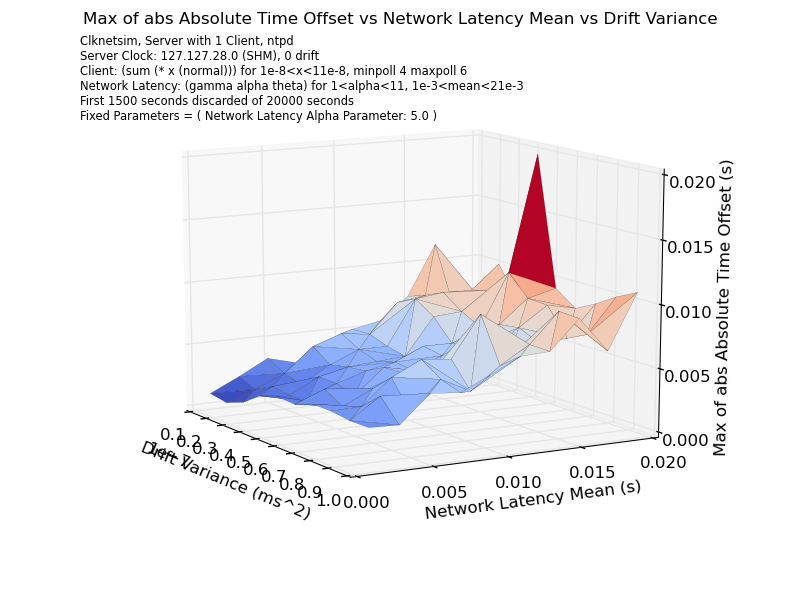
\includegraphics[width=0.8\linewidth]{max_abs_time-latency_mean-drift_var.png}
% \end{figure}

% \begin{figure}[h]
%   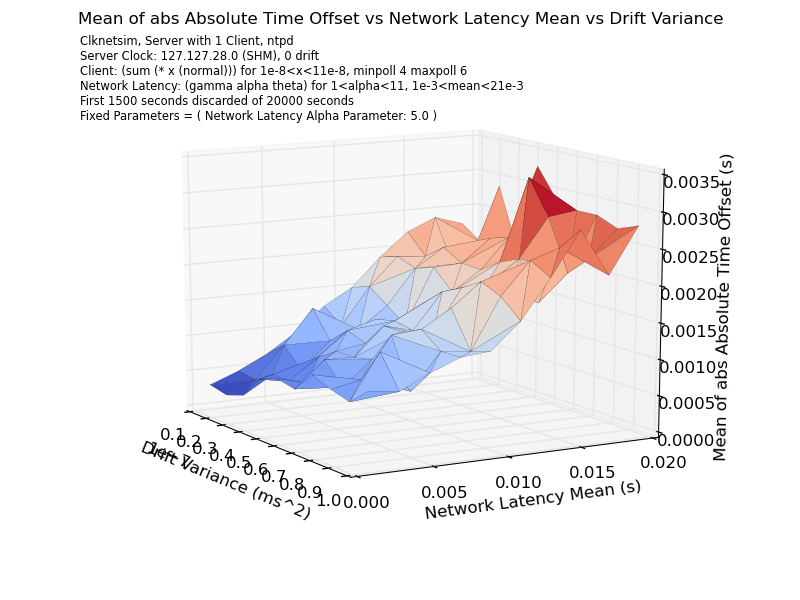
\includegraphics[width=0.8\linewidth]{mean_abs_time-mean_latency-drift_var.png}
% \end{figure}


%% Put these figures in an appendix
% \begin{figure}[h]
%   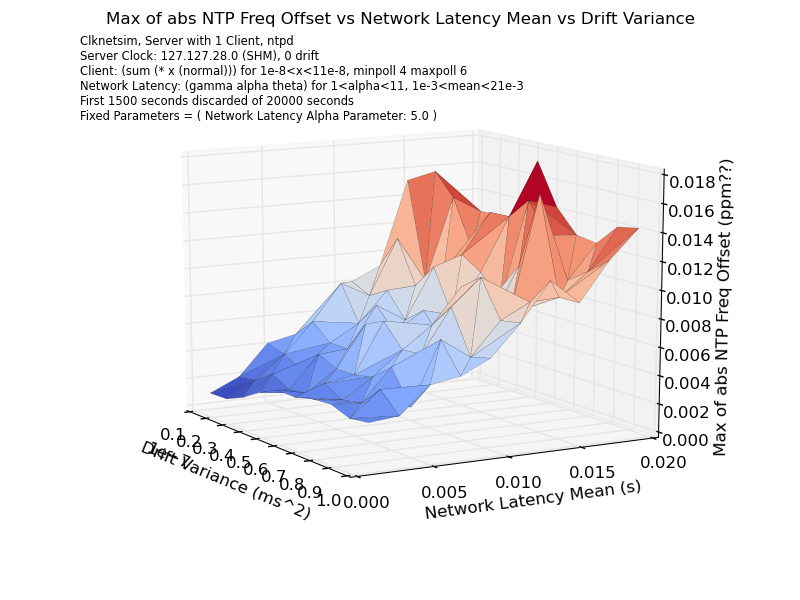
\includegraphics[width=0.8\linewidth]{max_abs_freq-mean_latency-drift_var.png}
% \end{figure}

% \begin{figure}[h]
%   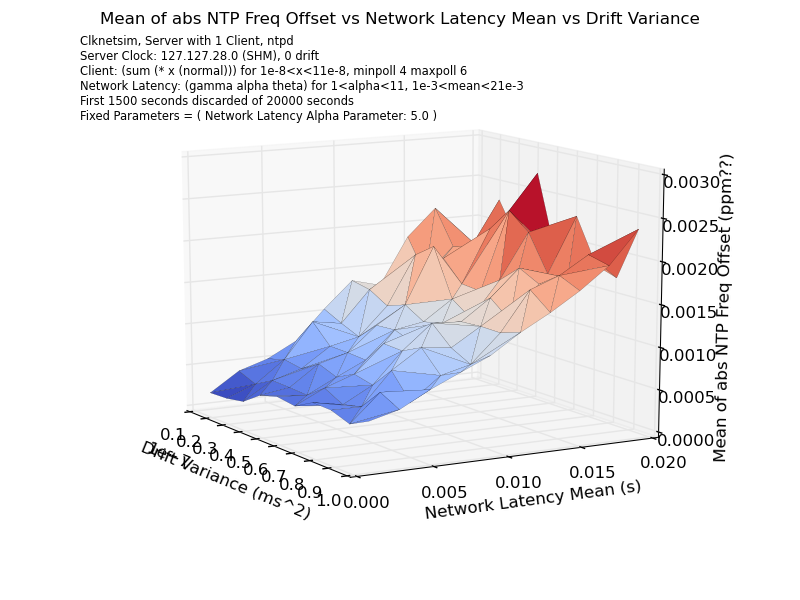
\includegraphics[width=0.8\linewidth]{mean_abs_freq-mean_latency-drift_var.png}
% \end{figure}

% \begin{figure}[h]
%   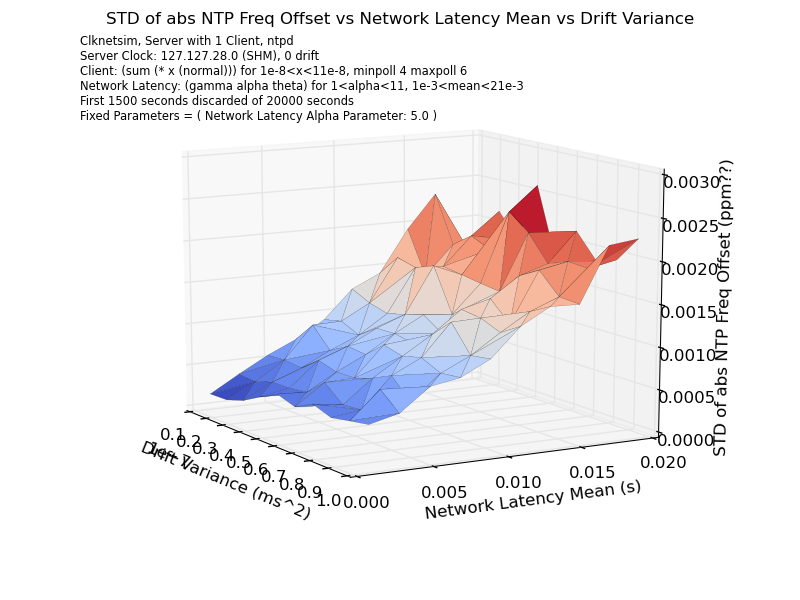
\includegraphics[width=0.8\linewidth]{stddev_abs_freq-mean_latency-drift_var.png}
% \end{figure}

% For larger variance in the drift, NTP does have to make larger
% frequency corrections, but it seems that NTP is more than capable of
% doing this, as these clock discipline corrections do not seem to
% translate into larger error or larger absolute time offsets. As the
% mean latency increases, NTP also seems to make larger frequency
% corrections. This likely means that, due to network asymmetries, NTP
% is more likely to over-correct or under-correct at times, resulting in
% an increase in the maximum offset. We also see that more normal
% latency distributions also result is smaller deviations in the
% frequency offset. The mean seems to not be significantly affected by
% either the latency or the drift variance, suggesting that most of the
% the clock frequency changes are the result of overcorrection and not
% the result of the clock actually keeping poor time. For graphs describing the 
% frequency offset values, see the appendix.

%% TODO: figure out which appendix this is going to be ^^

In summary, network latency mean has a large effect on the length of freeze 
windows. Latency value distribution does have an effect on freeze times, but
its effect is small in comparison to mean network latency. An
individual node's clock's drift variance is inconsequential to the
final performance of CASTS.

Uncertainties compound in NTP, thus it is advisable to acquire a
single, perfect clock to serve as a master. This will significantly
decrease the length of freeze windows.




%%% Section 7

\chapter{Analysis}
\label{sec:analysis}

\section{Correctness}

When we run our simulations, we want to determine whether NTP can give
accurate bounds on each node’s uncertainty range to include the real
time. This is the key characteristic of NTP that allows our algorithm
to work correctly.

At each node, NTP has an estimate for the real time and an uncertainty
in that estimate. Clknetsim allows us to access that information, and
it allows us to know the real time of the system. All of this allows
us to know what the “safety buffer” is for each node in real time.

The safety buffer, $S(t)$,  for a particular node is defined as:

\[ S(t) =U(t) - | t - E(t)| \]

where $t$ is the real time, $U(t)$ is NTP’s uncertainty in the real
time estimate for that node, and E(t) is NTP’s estimate for what the
real time is. In simpler terms, the safety buffer tells us where NTP’s
error in what the real time is lies within its uncertainty range (see
figure~\ref{fig:safety-diag}. If the safety buffer is a positive
value, then the difference between NTP’s estimate and real time is
within its uncertainty range. If it is negative, then it’s error is
outside of its uncertainty range, meaning that NTP doesn’t function as
we would expect.

\begin{figure}[h]
  \caption{} %% because label requires that it follow a caption in a fig
  \label{fig:safety-diag}
  \centering
  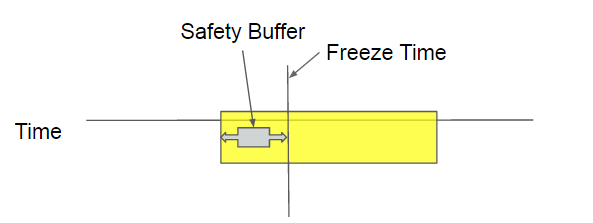
\includegraphics[width=0.8\textwidth]{safety-diagram.png}
\end{figure}

To prove the correctness of NTP, and therefore our algorithm, we ran a
Clknetsim simulation with 10 nodes over xxxxx %% TODO fill out your
section seconds, recording the safety buffer for each of the nodes at
every moment in time. We then aggregated those values for all of the
nodes together and we computed five points of data: the minimum value,
the maximum value, the average value, the average value plus one
standard deviation and the average value minus one standard
deviation. Those values are shown in figure~\ref{fig:safety-data}

\begin{figure}[h]
  \caption{}
  \label{fig:safety-data}
  \centering
  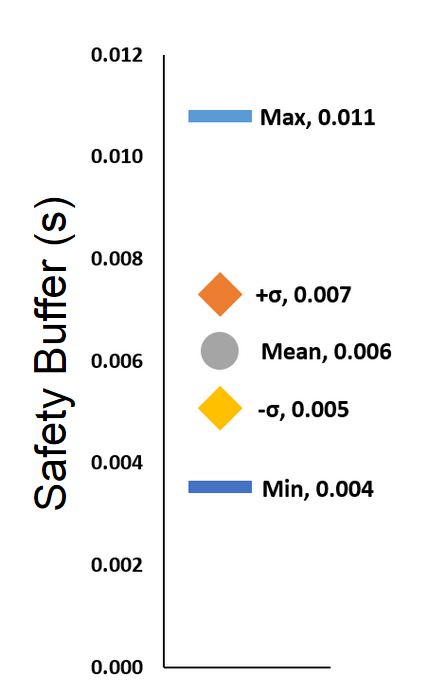
\includegraphics[width=0.8\textwidth]{safety-data.png}
\end{figure}

We can see that all of these values are positive. Since the minimum
value is a positive number, we can be sure that all of the values are
positive, which shows that NTP is functioning as we would
hope. Therefore, our algorithm can use NTP as a time synchronization
protocol.

\section{Performance}

Our testing has shown that NTP is a capable and resilient
algorithm. It seems likely that in any real-world network
configuration (baring hardware failure) NTP will be able to report
accuracy statistics that will result in the correct performance of our
algorithm. However, more exacting network layouts will be necessary to
make our algorithm performant. The data displayed in this section
summarizes trends seen when varying a number of parameters in a
standard network setup. We find few surprises -- network latency is
the standout determining factor for how performant our algorithm will
be. Lower the mean network latency and you will be rewarded by a
fairly consistently linear drop in freeze times.

It’s worth discussing how the network latency is modeled for these
simulations. Network latency was modeled using a gamma distribution,
since the data from the test Ceph cluster seemed to suggest that
latency approximately followed such a model. We varied two parameters:
the mean value and the shaping parameter, or alpha.

The shaping parameter represents how much of a tail our gamma
distribution has: a larger shaping parameter means that our gamma
distribution would have less of a tail. In the extremes, a small
shaping parameter approximates an exponential distribution and a large
shaping parameter approximates a normal distribution.

%% TODO please \ref these somewhere


\begin{figure}[h]
  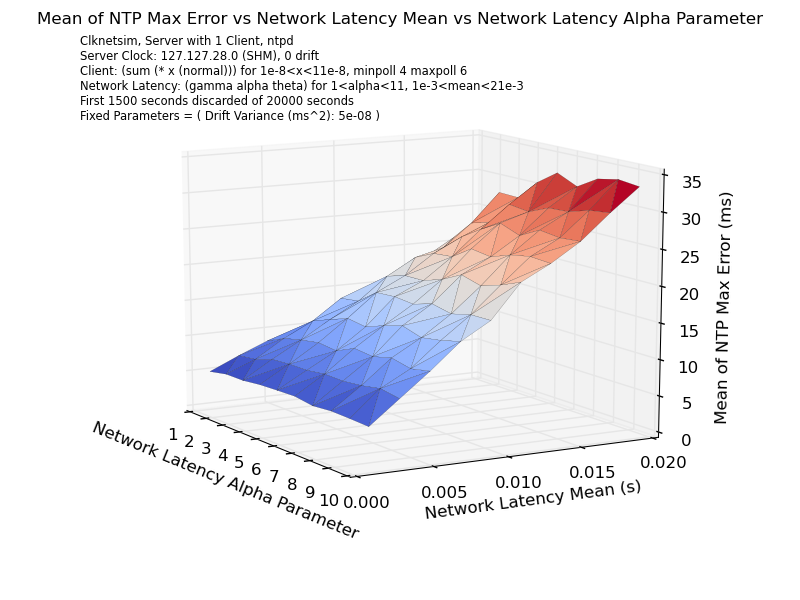
\includegraphics[width=1\linewidth]{mean_max_error-mean_latency-latency_alpha.png}
\end{figure}


\begin{figure}[h]
  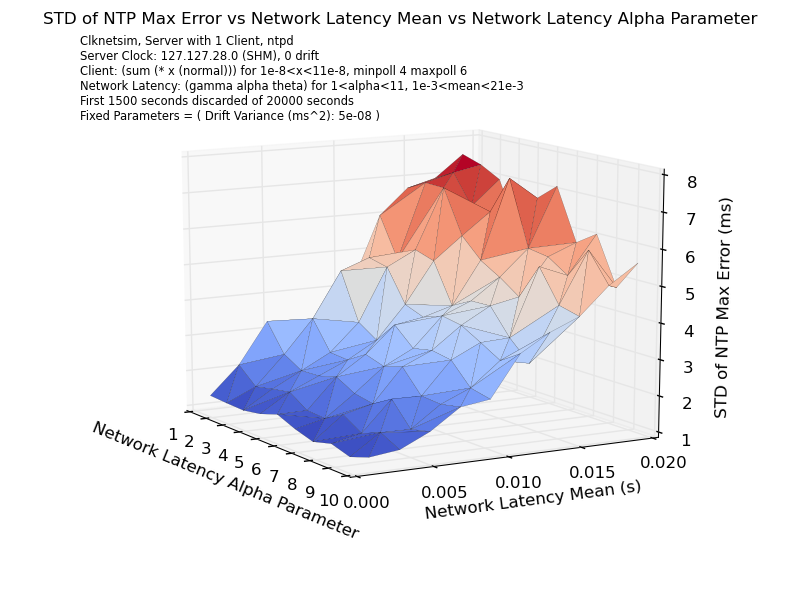
\includegraphics[width=1\linewidth]{max_err_stddev-latency_mean-latency_alpha.png}
\end{figure}

\begin{figure}[h]
  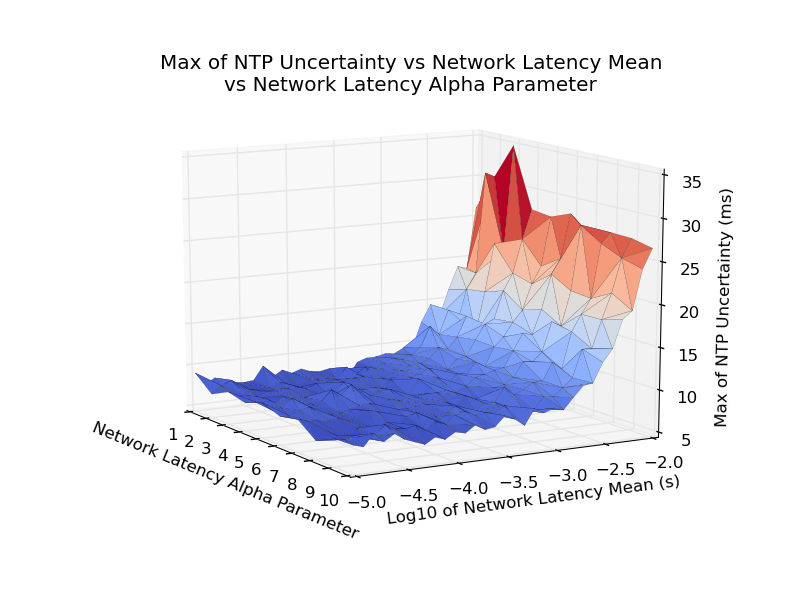
\includegraphics[width=1\linewidth]{max_error-latency_mean-latency_alpha.png}
\end{figure}

The NTP Max Error term is strongly affected by the mean network
latency. There is a much weaker effect on the Max Error by the shape
of the distribution of network latency traffic. NTP cares very little
about how the network tragic is distributed as long as the mean is
low. We can see in the upper right of MaxError vs Latency Mean vs
Alpha that there is a slight increase in Max Error for more
distributed latencies, especially as the mean latency grows.

Interestingly, we see that the mean of the max error term increases
with increasing alpha. This is likely because as alpha increases the
data become more normal. When the network latency distribution has a
long tail, most of our values will be less than or below the mean
value. Values larger and farther away from the mean tend to happen
less frequently and are more anomalous. Likely, NTP sees these values
are anomalies and ignores them, keeping its uncertainty at a lower,
more reasonable value. This explains why, for the graphs of the mean
and maximum of the error, we see lower values for lower alpha values.

As can be seen in figure~\ref{fig:max-mean-var-drift},
figure~\ref{fig:mean-mean-var-drift}, and
figure~\ref{fig:stddev-mean-drift-var} there is very little, if any,
effect of the drift variance of a node’s internal clock on the max
error term. This is expected network latency is a much larger term in
comparison to even the worst clocks. We again do see a strong,
apparently linear, correlation between mean latency and the max error
term. Looking at the mean of the max error term, we see values of
between 15 and 45 ms approximately. The max of the max error term for
any given run appears to be fairly predictable with few outliers in
the 20 to 70 ms range. The standard deviation of the measured max
error values is consistent with this, showing generally low
variability in the spread of max error values. We notice that the
spread does increase with increasing latency mean.

\begin{figure}[h]
  \caption{}
  \label{fig:max-mean-var-drift}
  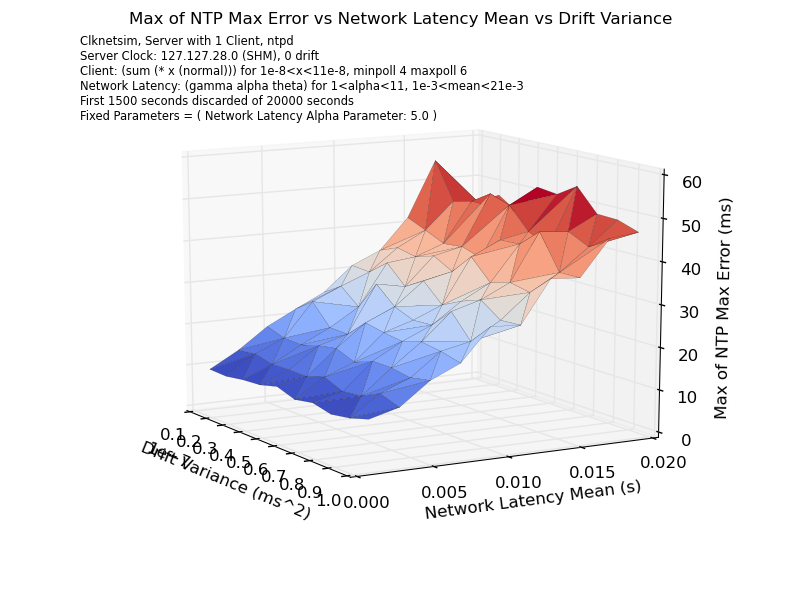
\includegraphics[width=1\linewidth]{max_max_err-mean_latency-drift_variance.png}
\end{figure}

\begin{figure}[h]
  \caption{}
  \label{fig:mean-mean-var-drift}
  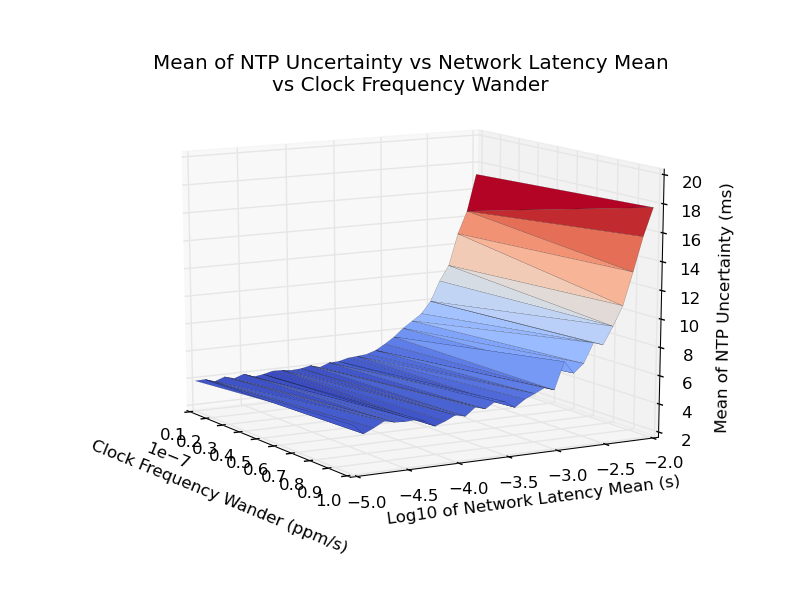
\includegraphics[width=1\linewidth]{mean_max_err-mean_latency-drift_variance.png}
\end{figure}

\begin{figure}[h]
  \caption{}
  \label{fig:stddev-mean-drift-var}
  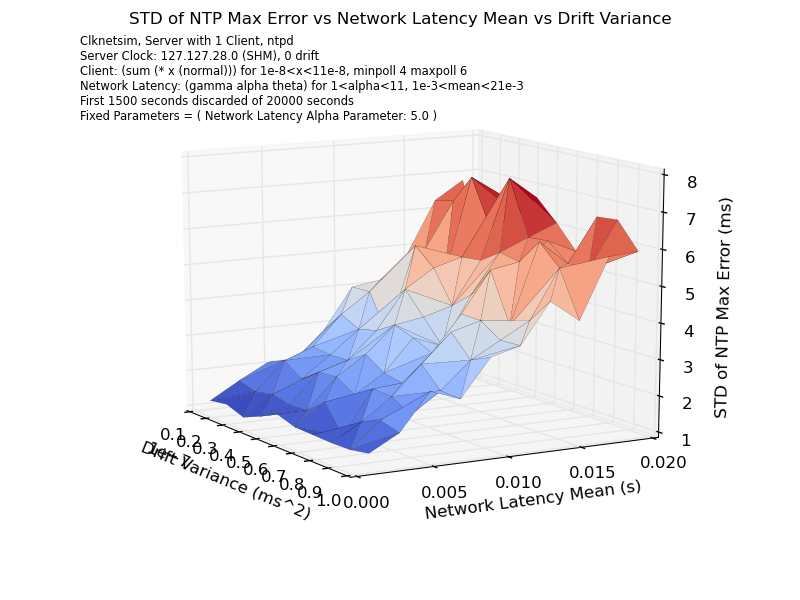
\includegraphics[width=1\linewidth]{stddev_max_err-mean_latency-drift_variance}
\end{figure}

Larger latency values do seem to mean that at any given time the
absolute time offset may be larger. However, network latency does not
seem to play a large role in the mean time offset. Drift seems to play
almost no role.

%% TODO please \ref these somewhere

\begin{figure}[h]
  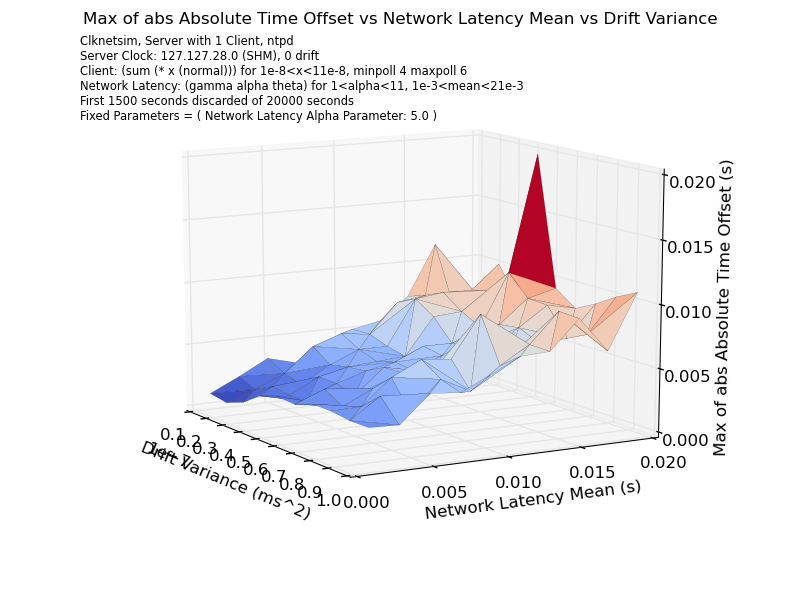
\includegraphics[width=1\linewidth]{max_abs_time-latency_mean-drift_var.png}
\end{figure}

\begin{figure}[h]
  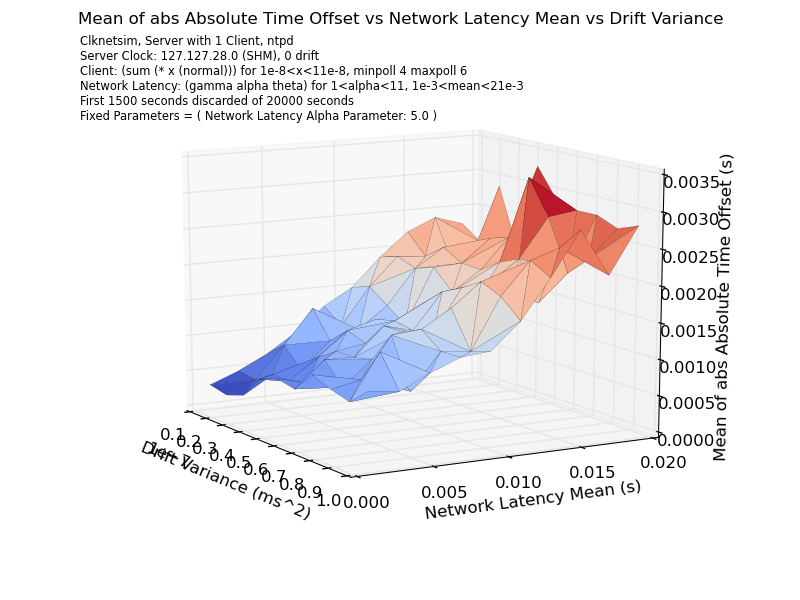
\includegraphics[width=1\linewidth]{mean_abs_time-mean_latency-drift_var.png}
\end{figure}

Larger latency values do seem to mean that at any given time the
absolute time offset may be larger. However, network latency does not
seem to play a large role in the mean time offset. Drift seems to play
almost no role.


%% TODO please \ref these somewhere

\begin{figure}[h]
  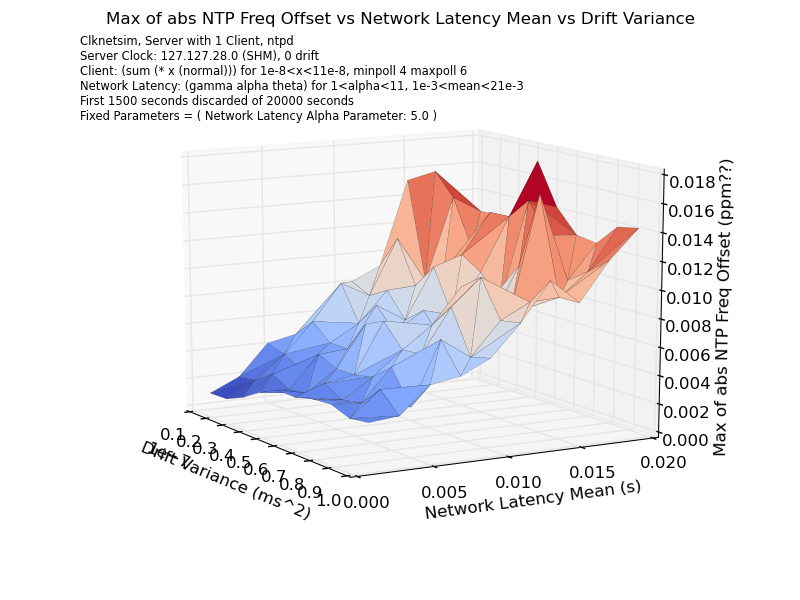
\includegraphics[width=1\linewidth]{max_abs_freq-mean_latency-drift_var.png}
\end{figure}

\begin{figure}[h]
  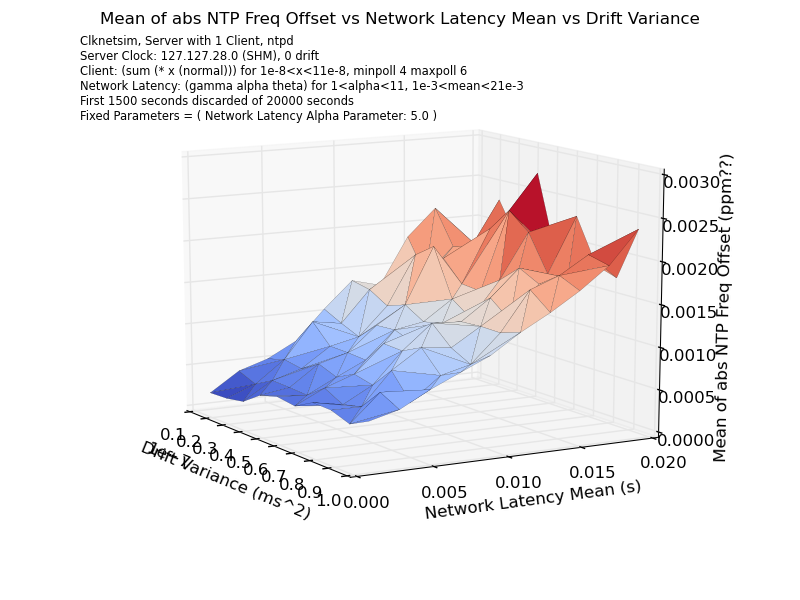
\includegraphics[width=1\linewidth]{mean_abs_freq-mean_latency-drift_var.png}
\end{figure}

\begin{figure}[h]
  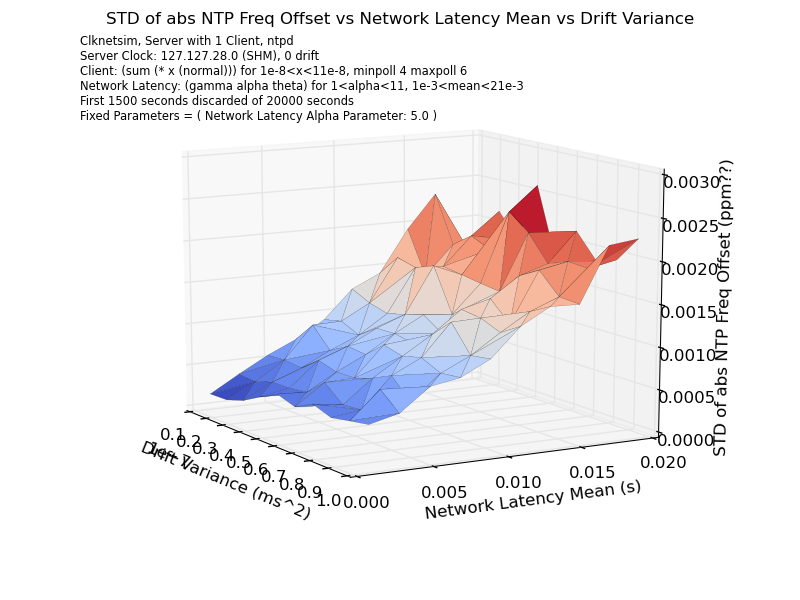
\includegraphics[width=1\linewidth]{stddev_abs_freq-mean_latency-drift_var.png}
\end{figure}

For larger variance in the drift, NTP does have to make larger
frequency corrections, but it seems that NTP is more than capable of
doing this as these clock discipline corrections do not seem to
translate into larger error or larger absolute time offsets. As the
mean latency increases, NTP also seems to make larger frequency
corrections. This likely means that, due to network asymmetries, NTP
is more likely to over correct or undercorrect at times, resulting in
an increase in the maximum offset. We also see that more normal
latency distributions also result is smaller deviations in the
frequency offset. The mean seems to not be significantly affected by
either the latency or the drift variance, suggesting that most of the
the clock frequency changes are the result of overcorrection and not
the result of the clock actually keeping poor time.

In summary, network latency mean has a larger effect on freeze
times. Network traffic shape does have an effect on freeze times, but
its effect is small in comparison to mean latency. An individual
node’s clock’s drift variance is inconsequential to the final
performance of our algorithm.

Due to how uncertainties compound in NTP, it is highly advisable to
acquire a single, good clock to serve as a master. This will
significantly decrease freeze windows.



%%% Section 8

\chapter{Implementation}
\label{sec:impl}

There are a few things to note about how implementation would work in
practice. First, NTP requires a few thousand seconds to settle,
because it not only works with last-seen error but also estimated
drift rate, changes in that drift rate. Thus, a new machine that is
being added to the cluster could not be used in snapshots until
roughly a few thousand seconds after it was added to the
cluster. Probably this would be handled by giving new machines a “warm
up” period before they are actually assigned data. Once the machine’s
NTP estimates settle, it can be incorporated into the Ceph cluster.

The quality of the master NTP clock significantly affects the size
required for safe freeze windows, as we saw in the simulation
results. We recommend that a GPS, atomic, or other highly precise
clock (any device capable as acting as an NTP stratum 0) be used
instead of the on-board RTC for that machine. This allows the master
clock to function as a stratum 1 clock, eliminating NTP uncertainty
due to upstream variation. This is not strictly necessary, and
performance is generally acceptable with a more distant stratum, but a
stratum 1 clock will provide the best performance for the
cluster. Without a stratum 0 device directly connect to the NTP
stratum 1 server, NTP is forced to assume to worst possible clock
properties for the on-board RTC.

Another time protocol could be used in place of NTP, and ideally one
more tailored to data center precision would in fact be usable. NTP
was used for analysis here because it is widely deployed, it can bound
its own uncertainty, and the reference implementation of the protocol
provides easy access to important diagnostic information. It is most
likely possible to implement the required uncertainty calculation in
PTP, but this would require extensions beyond the specification of the
protocol. Chrony, another NTP implementation, could likely also be
modified to report the necessary information.

There are a few fault conditions that can occur during a snapshot. The
simplest, the primary NTP master clock going down, would require a
short suspension of snapshotting (a few hundred to a few thousand
seconds, depending on the specific characteristics of the clocks)
until all clocks in the data center re-settled on the new master
clock. Scenarios with more than one master clock on a network have not
been analyzed.

\section{Snapshot Validation}

As in all systems, hardware failures are possible. As a result, we
must consider how to mitigate against a network disruption or clock
hardware failure leading to a significant clock desynchronization of
an individual or group of nodes. This would be detectable via a major
spike in various diagnostic outputs from NTP (different kinds of
uncertainty and measures of clock drift and wander. %% TODO explain this
The node would report this event either within a heartbeat message or
through an extra, priority message to one of the monitors. The
monitors would then be able to check that all of the failed node’s PGs
had replicas that did not experience such a failure. As shown in the
proof of correctness section, all correctly-behaving nodes have an
overlapping good time, so if at least one PG replica behaved
correctly, at least one would have prevented any writes from becoming
visible (the issue covered in the problem discussion TODO
REFERENCE). If there is at least one good node in each PG replica set,
the snapshot is still safe.



%%% Section 9

\chapter{Future Work}
\label{sec:future}

With our research and analysis, we have also found points of interest
should Red Hat or a future clinic team choose to pursue them. For one,
the algorithm proposed can be used with any time synchronization
protocol that provides guarantees on the clock uncertainty bounds. As
such, alternative time protocols such as Chrony or the Precision Time
Protocol (PTP) can be investigated to see if they could provide
tighter uncertainty bounds than NTP. As of the time of this writing,
those two particular protocols cannot provide guarantees on the
uncertainty bounds, but could possibly be extended to include them and
perhaps improve upon the bounds of NTP.

In addition, the algorithm proposed could be tested on a wider range
of scenarios than was done for this project to prove its
performance. The testing we did is more representative of smaller data
centers with a single NTP server for synchronization. Other tests
could include very large data centers, which would give more
uncertainty on the network latency values and, more importantly, use
more than one NTP server.

For our simulations, the model we currently use for clock drifting
behavior is a consistently normal distribution. Unfortunately, we were
unable to find literature describing better models for clock drifting
behavior. With further analysis and testing, a better model could be
found for clock drifting behavior to help analyze the performance of
the behavior. The clock drifting behavior is very dependent on
variables such as the Quartz crystal used, temperature and pressure
variance, and changes due to the synchronization process.



Lastly, our algorithm still needs to be implemented and incorporated
into Ceph. Our recommendations to approach this challenge are outlined
in section~\ref{sec:impl}. We believe that with a comfortable
understanding of the Ceph infrastructure, our algorithm could be
implemented without significant struggle.


%%% Section 10

\chapter{Conclusion}
\label{sec:conclusion}

The goal of our project was to design a snapshotting system for Ceph 
that allows for asynchronous replication of data to remote data centers.
We developed an algorithm that allows for taking these consistent, 
point-in-time snapshots by synchronizing clocks within a Ceph cluster
and performing short write holds for a length of time directly 
proportional to the uncertainty of the clock synchronization accuracy.
Even in the presence of out-of-band communication, the algorithm provides
consistency among all of the events even without external dependency
information. Our algorithm runs at the level of each individual node,
which means that a Ceph data center with this algorithm remains highly
scalable without increasing impact on the system. Also, with
reasonable guarantees on the uncertainty bounds provided by NTP, the
freeze windows, and as a result the snapshot, should have negligible
impact on a Ceph user. The algorithm is also robust to node failures
since as long as one replica of each node remains up, the snapshot can be
taken and the algorithm can succeed. We have found the NTP to be
satisfactory for the usage in our algorithm in fulfilling the problem
constraints, though we have also outlined alternatives and possible
future work for using and testing other time synchronization
protocols.



%%% Appendices.

%%% Appendices are just like chapters, only they're generally
%%% lettered rather than numbered (although that depends on your
%%% document class, of course).

%%% The appendices are delineated with the \appendix command.
%%% Individual appendices are begun with the standard \chapter or
%%% \section commands.  In our example, we'll \include them just as
%%% we did other chapters.

%%% If you don't have any appendices, comment out the \appendix
%%% command.

\appendix

\chapter{Initial Proposals for Plan of Action}
\label{sec:plan}

At beginning of the year, we proposed three possible plans of action
to our liaisons:

\begin{enumerate}

\item \emph{Viable Solution and Initial Integration}

  This would be the scenario where we had found a viable solution
  early enough in the academic year such that we would have had the
  time to both fully develop a final solution and to begin exploring
  how we would be able to integrate our solution into the current Ceph
  system. In this scenario, we would have found a viable solution
  sometime early in the fall semester. This would be after exploring a
  number of possible solutions and documenting why they were
  unsatisfactory. Our Midyear Report would contain details about what
  options we had explored, why they were unsatisfactory and a detailed
  explanation of what our solution was. It would also contain a proof
  that details why our solution is, theoretically, correct.

  The spring semester would be dedicated to creating a simulation data
  center that we could use to model an implementation of our
  solution. We would use a cluster of desktop machines or Raspberry
  Pis to simulate our solution to ensure that the constants on the
  runtime of our algorithm were not so large as to make our solution
  impossible to implement in real life. Finally, we would begin to
  look at the Ceph code base and see how we might be able to make
  recommendations about how to integrate our solution into Ceph's
  system. Our Final Report would contain a final description of all of
  the work done over the course of the school year, including the
  description of the solutions we considered, the reasons why those
  solutions were dismissed, the final solution and a proof of its
  correctness, a description of a simulation of the solution, and
  recommendations for how to incorporate the solution into the current
  Ceph system.


\item \emph{Viable Solution and Proof of Concept}

  This would be the case where we had found a viable solution later in
  the school year. While it would depend on when we finalized the
  solution, our Midyear Report would contain details about the
  algorithms that we had considered up to that point and a discussion
  about the drawbacks of the ones we discarded. Depending on when we
  had found a viable algorithm, we may have included in that document
  a description of the algorithm and a proof of the correctness of
  that algorithm.

  The spring semester would be about proving that our solution is
  viable. We would create the proof of correctness, if we hadn't
  already done it in the fall semester and we would create and run the
  simulations of our algorithm on an imitation cluster. Our Final
  Report would contain a final description of all of the work done
  over the course of the school year, including the description of the
  solutions we considered, the reasons why those solutions were
  dismissed, the final solution, a proof of its correctness and a
  description of a simulation of the solution.


\item \emph{In-Depth Exploration of Ideas}

  The last scenario was the case where we are unable to find a
  solution. In that case, our goal would be to lay as much groundwork
  as we could for a future clinic team to take over after we
  finish. In the fall semester, we would do a significant amount of
  research into related work. We would try to apply the related work
  to come up with a solution and we would discuss all of the options
  that we considered and found were unsatisfactory. Our midyear report
  would contain all of the insights we gleaned over the semester,
  including the possible solutions that we explored and the reasons we
  decided they were unsatisfactory.

  In the spring semester, we would spend most of our time working on
  possible solutions, since we had spent most of the previous semester
  doing research. Our goal would be to come up with as many algorithms
  as we could and analyze the pros and cons of each of them. The Final
  Report would be devoted to describing the different algorithms and
  pieces of related work that we looked at over the year. We would
  also provide details into why the solutions that we looked at were
  unsatisfactory. The goal would be to create a document that provides
  a future clinic team with a good foundation to take up this project
  after us.

\end{enumerate}

We completed the goals of the second plan. 


\chapter{Commonly Used Terms}
\label{sec:terms}

\section{General terms}
\begin{itemize}

\item Cluster: Computers that are networked together to perform a
  common task. A Ceph cluster is a single deployment of the Ceph file
  system across a group of computers.
    
\item Clock Drift: The natural drift over time that a computer clock
  experiences.
    
\item Clock Wander: The rate of clock drift.

\item Consistency: The partial ordering of events to preserve the
  causal relationships between them.
    
\item Node: A single computer in a cluster.
  
\item Node Failure: When a node in the cluster becomes unavailable,
  either temporarily or permanently.
      
\item Node Freeze: A hold on processing all writes that are sent to
  that node. Reads may continue to be processed.
    
\item Node Time: The time that the clock on a particular node reads;
  it is not guaranteed to be the same as real time, although we hope
  it is close.
    
\item Out-of-Band Communication: Communication between users of a Ceph
  cluster that Ceph has no way of detecting or recording.
    
\item Real Time: The true, global time of the cluster. This can be
  considered the time advertised by a standards organization or a
  perfect clock.

\item Snapshot: A consistent recording of the entire state of a Ceph
  cluster.  This includes the state of files and objects stored within
  the cluster.
    
\item Strong Consistency: Ceph is strongly consistent. It requires
  that ordering of events be maintained even in the face of
  out-of-band communication. It also requires that data stored in the
  cluster will be returned correctly when asked for or be
  unavailable. It does not allow data to be returned corrupt.

\item Time Synchronization Protocol: A protocol that the nodes in a
  cluster implement to synchronize their clocks as they drift.


  
\end{itemize}




%%% Back matter.

%%% The back matter of a document is where the bibliography, index,
%%% glossary, and other unnumbered chapters or sections occur.  It
%%% starts, not surprisingly, with the \backmatter command.

\backmatter


%%% Bibliography.

%%% BibTeX is the tool to use for citations and layout of your
%%% bibliography.  Instead of having to type ``[5]'' or ``(Jones,
%%% 1968)'' (and keep track of which citation is which and renumber
%%% them as you add more references to your bibliography), you use
%%% special commands that allow BibTeX and LaTeX to automatically put
%%% the correct information in the right place.

%%% Depending on your field, it may or may not be appropriate to list
%%% references for which you haven't included specific citations.  If
%%% your field sanctions such practices, or if you just want to get an
%%% idea of what you have in your bibliography file, you can include
%%% everything with the \nocite{*} command.
\nocite{*} 


%%% The appearance of your bibliography and citations in your text are
%%% defined by a combination of any bibliography-related LaTeX
%%% packages (such as natbib, harvard, or chicago) and the particular
%%% bibliography style file that you load with the \bibliographystyle
%%% command.  Bibliography-style files end in .bst; you can find them
%%% by searching your file system using whatever tools you have for
%%% doing searches.  (On most modern Unices, ``locate .bst'' will give
%%% you an idea of what's available.)

% Standard bibliography style.
\bibliographystyle{hmcmath}

% Annotated bibliography style.
% \bibliographystyle{hmcmathannote}


%%% The particular bibliography data file or files that you want to
%%% use are specified with the \bibliography file.  Multiple files are
%%% separated by commas.

%%% You might want to use multiple bibliography (or ``bib'') files if
%%% you had a master bib file containing references you use again and
%%% again, and another containing only records for references for a
%%% particular project.

%%% Many people create a single, large bib file that they use for
%%% everything they write.  That approach requires you to \cite every
%%% reference that you want to use in your document -- using
%%% \nocite{*} with a huge bibliography database will give you a large
%%% bibliography containing many references you haven't consulted for
%%% your particular document!

\bibliography{clinic-papers}


%%% Glossary or Index.

%%% If you were going to include a glossary or index in your document,
%%% the relevant commands would appear here.

%%% If you think that you would like to include such features, talk
%%% with someone who's worked with LaTeX a lot very early in your
%%% writing process.  These commands require you to do a bit of
%%% thinking about what you would want to index or gloss in
%%% advance---going back though a completed document to add \index
%%% commands is *not fun*.


\end{document}


